\chapter{Wprowadzenie teoretyczne}
\section{Wykorzystywane terminy}
\label{sec:terminy}
W niniejszej pracy, posłużono się terminologią dystynktywną z punktu widzenia realizacji, rozwoju oraz ewaluacji usług sieciowych. Najbardziej istotne spośród wykorzystywanych terminów wymieniono poniżej. Dla każdego z pojęć przedstawiono obcojęzyczne tłumaczenie, a także zdefiniowano spójny oraz zwięzły opis.

\subsection*{Usługa sieciowa}
\subsubsection{\textit{Web Service}}
Rodzaj systemu informatycznego cechującego się permanentnym wykonywaniem zdefiniowanych funkcji tuż po uzyskaniu żądania. Żądanie to, przybiera postać danych przekazanych w ramach systematycznej struktury. Sposób dostarczenia żądania, jego format, a także metoda odpowiedzi na żądanie definiowane są poprzez protokół sieciowy z którego korzysta dana usługa.

\subsection*{Interfejs Programowania Aplikacji}
\subsubsection{\textit{Application Programming Interface}}
Zbiór reguł oraz struktur programistycznych określający metodę oraz cel interakcji pomiędzy komponentami oprogramowania. Pojęcie interfejsu programowania aplikacji jest niezależne od warstwy implementacji systemu i może tyczyć się dowolnego rodzaju programu komputerowego. Interfejs API definiowany jest na poziomie kodu źródłowego poszczególnych fragmentów oprogramowania a jego zadaniem jest dostarczenie wymaganych specyfikacji struktur programistycznych, a także protokołu pozwalającego na ich wykorzystanie przez zewnętrzny komponent programowy.  

\subsection*{API wykonane w technologii REST}
\subsubsection{\textit{RESTful API}}
Interfejs programowania aplikacji bazujący zarówno w swojej strukturze jak i funkcjonalności na zbiorze ściśle określonych reguł dostarczanych w ramach metodologii REST. Reguły metodologii tej implementowane są najczęściej w stosunku do interfejsów programowania aplikacji, które wykorzystują w kontekście zewnętrznej komunikacji protokół hipertekstowy. Podstawowa charakterystyka interfejsu programowania aplikacji opartego o zbiór reguł REST definiowana jest poprzez bezstanowość transmisji danych, pojęcia zasobów i reprezentacji, a także cechę jednolitości interfejsu komunikacyjnego.

\subsection*{Kontroler}
\subsubsection{\textit{Controller}}
Struktura programistyczna (w przypadku języków programowania opartych o paradygmat obiektowy klasa), której celem jest obsługa żądania dostarczonego od aplikacji klienckiej, zweryfikowania zgodności jego treści a następnie przekierowanie wykonania programu do odpowiedniej metody warstwy logiki biznesowej.
Po zakończeniu wszystkich operacji dotyczących omawianego zapytania metoda dostępna w ramach klasy kontrolera formułuje odpowiedź zwracaną bezpośrednio do konsumenta żądania.

\subsection*{Serwis}
\subsubsection{\textit{Service}}
Struktura programistyczna (w przypadku języków programowania opartych o paradygmat obiektowy klasa), której zadaniem jest realizacja obliczeń związanych z określonym obiektem lub domeną, w ramach której określony obiekt się znajduje. Klasy serwsisów (nazywane również klasami logiki biznesowej) stanowią centralny punkt przetwarzania w ramach interfejsów programowania aplikacji, a także pełnią rolę pośrednika pomiędzy komponentami odpowiedzialnymi za zarządzanie żądaniem (tj. metodami kontrolerów) oraz pozyskiwanie danych z określonych źródeł (tj. metodami repozytoriów).

\subsection*{Repozytorium}
\subsubsection{\textit{Repository}}
Struktura programistyczna (w przypadku języków programowania opartych o paradygmat obiektowy klasa), której rolą jest wykonywanie operacji na obiektach modelu danych komunikując się bezpośrednio z wykorzystywanym systemem bazodanowym. Operacje zawarte wewnątrz metod klas repozytoriów mogą mieć postać kwerend lub komend definiowanych w języku zapytań dostarczanym przez serwer bazodanowy. Mogą również operować na dostępnej w pamięci aplikacji strukturze danych bądź też odwoływać się do zewnętrznego zbioru bazodanowego manipulując instancjami klas zdefiniowanego wewnątrz aplikacji modelu. W ostatnim z omawianych przypadków, aktualizacje wartości w ramach encji modelu danych są identyfikowane przez maper obiektowo-relacyjny, który generuje polecenia języka zapytań systemu bazodanowego mające na celu synchronizację stanu danych aplikacji oraz zewnętrznego źródła informacji. Metody klas repozytoriów są wywoływane wewnątrz metod logiki biznesowej.

\subsection*{Mapper obiektowo-relacyjny}
\subsubsection{\textit{Object-relational mapper}}
Oprogramowanie, którego głównym zadaniem jest konwersja struktury klas modelu danych do fizycznej organizacji tabel w ramach systemu bazodanowego. Ponadto, mapper obiektowo-relacyjny dostarcza zbiór właściwości oraz metod stanowiących fasadę dla niskopoziomowych procedur dostępu do bazy danych, a także modyfikacji danych w niej zawartych.

\subsection*{Pamięć podręczna}
\subsubsection{\textit{Cache}}
Wydzielony fragment pamięci cechujący się szybkim czasem dostępu, wysoką przepustowością transmisji, a także ograniczonym okresem trwałego przechowywania danych. Pamięć ta, w kontekście webowego interfejsu programowania aplikacji wykorzystywana jest w celu przechowywania wyników często realizowanych operacji, a także magazynowania uprzednio dostarczonych do klienta fragmentów odpowiedzi na żądania.

\subsection*{Przetwarzanie współbieżne}
\subsubsection{\textit{Concurrent Computing}}
Technika programistyczna oparta o wykorzystanie wielu współistniejących procesów oraz wątków dostępnych w obrębie jednej aplikacji, a także odwołujących się do współdzielonych struktur danych. Poszczególne wątki stanowią elementy składowe pojedynczego procesu i są uruchamiane na tej samej centralnej jednostce przetwarzania. Procesor wykonuje operacje przełączania pomiędzy kontekstami poszczególnych wątków dzięki czemu uzyskać można wrażenie, że wykonania wielu spośród tych elementów odbywają się w sposób równoległy. Z punktu widzenia interfejsu programowania aplikacji, który implementuje technikę przetwarzania współbieżnego wyróżnić możemy punkty końcowe, które definiowane są jako osobne wątki aplikacji. Dlatego też interfejs programowania aplikacji cechuje się dostępnością pomimo jednoczesnego przetwarzania wielu niekiedy długotrwałych żądań klientów.

\subsection*{Algorytm metaheurystyczny}
\subsubsection{\textit{Metaheuristic algorithm}}
Technika projektowania algorytmów nie zapewniających gwarancji uzyskania optimum dla rozważanego problemu jednakże pozwalająca na zbudowanie systemu dostarczającego rozwiązanie złożonego zagadnienia w akceptowalnym czasie, a także uzyskiwanego przy wykorzystaniu akceptowalnej ilości zasobów sprzętowych. Algorytm metaheurystyczny poza konwencjonalnymi regułami stosowanymi w ramach standardowych wzorców programowania implementuje reguły rozwiązywania problemów oparte na losowości bądź też wywnioskowane na podstawie zjawisk fizycznych.

\subsection*{Punkt końcowy interfejsu programowania aplikacji}
\subsubsection{\textit{API Endpoint}}
Punkt końcowy usługi sieci web definiuje jeden z końców kanału komunikacyjnego pomiędzy aplikacją kliencką a serwerową. W momencie interakcji interfejsu programowania aplikacji z odrębnym systemem punkt styku dwóch usług sieciowych w ramach omawianej interakcji nazywany jest punktem końcowym. W odniesieniu do wewnętrznej struktury interfejsu programowania aplikacji, punkt końcowy wywołuje związaną z nim metodę klasy kontrolera a samo powiązanie identyfikowane jest (w przypadku usługi sieciowej bazującej na protokole hipertekstowym i metodologii REST) poprzez nazwę zasobu, rodzaj metody, a także parametry żądania.

\subsection*{Żądanie realizowane w ramach usługi protokołu hipertekstowego}
\subsubsection{\textit{HTTP Request}}
Struktura danych wysyłana od aplikacji klienckiej (tj. aplikacji internetowej, przeglądarki, czy też programu klienta HTTP) w kierunku usługi sieciowej. Żądanie protokołu hipertekstowego charakteryzuje się jednoznacznie zdefiniowaną strukturą uwzględniającą m.in. unikalny identyfikator zasobu, listę zdefiniowanych nagłówków, ciało żądania oraz jedną z dziewięciu dopuszczalnych metod HTTP. 

\subsection*{Odpowiedź usługi protokołu hipertekstowego}
\subsubsection{\textit{HTTP Response}}
Struktura danych wysyłana przez usługę sieciową w kierunku aplikacji klienckiej. Odpowiedź HTTP ma na celu poinformowanie klienta serwisu webowego o statusie realizacji wysłanego przez niego uprzednio żądania. Podstawowymi elementami odpowiedzi usługi protokołu hipertekstowego są: ciało odpowiedzi (zdefiniowane najczęściej z wykorzystaniem notacji JSON lub języka XML), kod odpowiedzi (liczba determinująca stan wykonania żądania), a także zbiór informacji nagłówkowych dotyczących typu danych zawartych w odpowiedzi czy też fizycznych informacji o serwerze usługi sieciowej.

\subsection*{Kod odpowiedzi usługi protokołu hipertekstowego}
\subsubsection{\textit{HTTP Response Code}}
Liczba determinująca status realizacji żądania wysłanego przez aplikację kliencką. Kod odpowiedzi stanowi jedną z wymaganych składowych dotyczących standardowego rezultatu zwracanego w ramach usługi opartej o protokół hipertekstowy. Wyróżnić możemy pięć kategorii kodów odpowiedzi niosących ze sobą odmienną informacje. Kategoriami tymi są: kody informacyjnej odpowiedzi (100--199), kody poprawnej odpowiedzi (200--299), kody wiadomości o przekierowaniu (300--399), kody błędu aplikacji klienckiej (400--499) oraz kody błędu aplikacji serwerowej (500--599).

\subsection*{Czas odpowiedzi usługi protokołu hipertekstowego}
\subsubsection{\textit{HTTP Response Time}}
Wyrażony w milisekundach przedział czasu od momentu otrzymania żądania wygenerowanego przez aplikację kliencką do chwili zwrócenia rezultatu wykonywanych przez usługę sieciową obliczeń. Liczba ta stanowi jedną z wartości pomiarowych w kontekście której rozpatrywana jest efektywność działania interfejsu programowania aplikacji.  

\subsection*{Obiektowa notacja JavaScript}
\subsubsection{\textit{JavaScript Object Notation -- JSON}}
Format definicji, reprezentacji, a także wymiany danych w postaci obiektów niezależny od określonego języka programowania. Obiektowa notacja JavaScript jest powszechnie wykorzystywana jako format komunikatów przekazywanych pomiędzy interfejsami programowania aplikacji a systemami klienckimi. W odróżnieniu od języka reprezentacji danych opartego o znaczniki \textit{Extensible Markup Language -- XML}, obiektowa notacja JavaScript cechuje się mniejszym rozmiarem przesyłanych obiektów (poprzez redukcję liczby metadanych), jednolitym standardem niezależnym od technologii, a także brakiem przechowywania informacji o typie poszczególnej wartości zadanego obiektu.

\subsection*{Testy wzorcowe}
\subsubsection{\textit{Benchmark}}
Rodzaj ewaluacji oprogramowania, której zadaniem jest określenie referencyjnego poziomu wydajności dla testowanego systemu. Metryki uzyskane w ramach testów wzorcowych mogą zostać wykorzystane jako wartości ograniczeń względem testów obciążeniowych oraz przeciążeniowych. 

\subsection*{Testy dymne}
\subsubsection{\textit{Smoke testing}}
Metoda testowania oprogramowania, której celem jest sprawdzenie poprawności funkcjonowania poszczególnych elementów systemu. Testy dymne wykonywane są przed testami wydajnościowymi po to aby upewnić się co do braku błędów implementacyjnych w ramach analizowanego oprogramowania.

\subsection*{Testy wydajności podstawowej}
\subsubsection{\textit{Baseline performance testing}}
Metoda ewaluacji oprogramowania pozwalająca na weryfikację działania systemu w warunkach analogicznych do realiów standardowego działania. Na podstawie testów wydajności podstawowej określić można wartości metryk, które będą miały zastosowanie jako punkt odniesienia dla kolejnych rodzajów testów. Ponadto, wykorzystując standard pomiaru wydajności aplikacji internetowych (taki jak np. APDEX) wartości uzyskane w ramach ewaluacji podstawowych mogą posłużyć w celu określenia punktów satysfakcji, tolerancji oraz frustracji.

\subsection*{Testy obciążające}
\subsubsection{\textit{Load testing}}
Rodzaj testów, które mają na celu określenie maksymalnego poziomu natężenia operacji jakie mogą być generowane w kierunku oprogramowania. W kontekście niniejszej pracy operacjami tymi są żądania wysyłane do interfejsu programowania aplikacji. Kluczowym aspektem testu obciążeniowego jest zdefiniowanie progu obciążenia aplikacji powyżej którego system jest nie w stanie generować poprawnych odpowiedzi w akceptowalnym czasie.

\subsection*{Testy przeciążeniowe}
\subsubsection{\textit{Stress testing}}
Metoda ewaluacji oprogramowania w ramach której natężenie operacji generowanych w kierunku testowanego oprogramowania zwiększone jest ponad ustalony próg tolerancji. Celem testu przeciążeniowego jest obserwacja sposobu działania systemu w momencie, w którym nie jest on w stanie przetwarzać otrzymywanych żądań w sposób poprawny.

\subsection*{Asercja}
\subsubsection{\textit{Assertion}}
Wyrażenie typu prawda/fałsz zdefiniowane w dowolnym miejscu programu, które przyjmuje wartość prawdziwą w momencie spełnienia hipotezy zawartej w ramach określonego przypadku testowego. Praktyczne podejście do procesu testowania funkcjonalności oprogramowania sprowadza się do definiowania hipotez oraz ciągów operacji w kontekście przypadków testowych a następnie weryfikacji tych hipotez z wykorzystaniem asercji.

\section{Interfejsy programowania aplikacji}
\label{sec:api-teoria}
Webowy interfejs programowania aplikacji to usługa sieciowa, której celem jest realizacja zadań zleconych przez oprogramowanie klienta. Zadania te dotyczą operacji wykonywanych w kontekście określonych zasobów. Wyróżnić możemy operacje zwane zapytaniami (tj. dotyczące pozyskiwania danych z ich źródeł), a także komendami (tj. związane z wykonywaniem operacji na danych).

Interfejsy API budowane są z wykorzystaniem protokołu HTTP dlatego też w ich kontekście możemy mówić o komunikacji bezstanowej definiującej pojęcia żądania oraz odpowiedzi. W związku z charakterystyką protokołu hipertekstowego zarówno żądanie jak i odpowiedź cechuje się regularną strukturą zawierającą predefiniowane elementy.

Żądanie protokołu http wysyłane jest od aplikacji klienta do interfejsu API. Podstawową składową tego polecenia stanowi unikalny identyfikator zasobu URI (\textit{ang. Uniform Resource Identifier}) na podstawie którego możliwe jest określenie fragmentu dziedziny obsługiwanego modelu danych. Informacja ta jednak nie jest wystarczająca w kontekście realizacji jednej z funkcjonalności zdefiniowanych w ramach API. Żądanie klienta musi zostać uzupełnione o jedną z dziewięciu ustalonych metod http obsługiwaną wersję protokołu a także zbiór linii nagłówkowych. Opcjonalnie informacja wysyłana w kierunku interfejsu może zostać wzbogacona o zawartość tekstową określaną ciałem żądania (\textit{ang. Request body}). Taki zbiór informacji pozwala na jednoznaczną identyfikacje fragmentu kodu programu, który ma zostać wykonany wewnątrz interfejsu programowania aplikacji. W tabelach \ref{tab:metody-http} oraz \ref{tab:naglowki-zadanie} przedstawiono kolejno listę zdefiniowanych metod protokołu hipertekstowego wraz z wyjaśnieniem ich przeznaczenia, a także zbiór najczęściej wykorzystywanych linii nagłówkowych w kontekście realizacji żądań.

\begin{longtable}{|l|p{12cm}|}
    \caption{Zbiór dozwolonych metod protokołu hipertekstowego}
    \label{tab:metody-http} \\
    \hline
    Nazwa metody & Opis \\ \hline\hline
    \endhead
    GET &
      Pozyskanie danych dotyczących pojedynczej instancji określonego zasobu lub grupy instancji z opcjonalnym uwzględnieniem warunków kwalifikacji poszczególnej instancji do grupy. \\ \hline
    POST &
      Definiowanie nowej instancji dotyczącej określonego typu zasobu. Przy zastosowaniu metody POST, wymagane jest zdefiniowanie ciała żądania, jako części składowej generowanej instrukcji. \\ \hline
    PUT &
      Aktualizacja pełni zawartości instancji występującej w ramach odwołania się do określonego zasobu. Przy zastosowaniu metody PUT, wymagane jest zdefiniowanie ciała żądania, jako części składowej generowanej instrukcji. \\ \hline
    DELETE &
      Usunięcie istniejącej instancji dotyczącej określonego typu zasobu. \\ \hline
    PATCH &
      Aktualizacja fragmentu zawartości instancji występującej w ramach odwołania się do określonego zasobu. Przy zastosowaniu metody PATCH, wymagane jest zdefiniowanie ciała żądania, jako części składowej generowanej instrukcji. \\ \hline
    HEAD &
      Pozyskanie zbioru linii nagłówkowych, które byłyby dostarczone wraz z ciałem odpowiedzi w ramach żądania wykorzystującego metodę GET. Wygenerowanie żądania HEAD umożliwia określenie charakteru danych, przed ich ewentualnym pozyskaniem. \\ \hline
    OPTIONS &
      Pozyskanie informacji dotyczących charakterystyki oraz struktury serwera. Definiując żądanie typu OPTIONS, klient może dowiedzieć się o dopuszczalnych metodach HTTP obsługiwanych przez serwer, czy też uzyskać informacje o nazwie serwera oraz wykorzystywanym systemie operacyjnym. \\ \hline
    CONNECT &
      Ustanowienie dwukierunkowej komunikacji pomiędzy klientem a serwerem. W przypadku realizacji komunikacji szyfrowanej, żądanie typu CONNECT pozwala na zestawienie zabezpieczonego tunelu pomiędzy hostami. \\ \hline
    TRACE &
      Wygenerowanie komunikatu diagnostycznego w ramach pętli zwrotnej, którego celem jest osiągnięcie każdego z hostów, biorących udział w komunikacji. \\ \hline
\end{longtable}

\begin{longtable}{|l|p{6cm}|p{5cm}|}
    \caption{Zbiór najczęściej wykorzystywanych linii nagłówkowych w kontekście żądania protokołu hipertekstowego}
    \label{tab:naglowki-zadanie} \\
    \hline
    Linia nagłówkowa & Znaczenie & Dopuszczalna zawartość \\ \hline\hline
    \endhead
    accept & Typ zawartości, którą jest w stanie przetwarzać aplikacja kliencka & Identyfikator typu MIME (\textit{ang. Multipurpose Internet Mail Extensions}) lub zapis */* oznaczający dowolną zawartość  \\ \hline
accept-encoding & Sposób kodowania znaków, rozumiany przez stronę klienta & Zbiór formatów kodowania zdefiniowany w ramach rejestru formatów IANA\\ \hline
accept-language & Język naturalny, preferowany przez stronę kliencką & Pojedyncza wartość reprezentująca określony kraj lub region, bądź też lista niniejszych wartości wraz z parametrem istotności poszczególnego kodu lokalizacji\\ \hline
content-length & Długość ciała żądania wyrażona w bajtach & Liczba naturalna\\ \hline
content-type & Format zawartości ciała żądania & Identyfikator typu MIME wraz ze sposobem kodowania wiadomości\\ \hline
cookie & Zbiór informacji pozwalających na wprowadzenie oraz utrzymanie stanowego charakteru transmisji & Zestaw par klucz-wartość, gdzie klucz jest wartością tekstową, a wartość przyjmuje postać dowolną\\ \hline
origin & Informacja determinująca pochodzenie żądania & Ciąg tekstowy składający się z nazwy protokołu, nazwy hosta oraz numeru portu\\ \hline
user-agent & Specyfikacja techniczna oprogramowania klienta & Ciąg znaków zawierający informacje o nazwie produktu, jego wersji, platformie sprzętowej, czy też systemie operacyjnym \\ \hline
\end{longtable}

Po wykonaniu kodu programu przypisanego do określonego rodzaju polecenia generowanego przez aplikacje kliencką z interfejsu programowania aplikacji zwracana jest odpowiedź na żądanie (\textit{ang. HTTP response}). Analogicznie do instrukcji realizacji danej czynności także odpowiedź dotycząca statusu jej wykonania jest ustrukturyzowana zgodnie z wytycznymi zawartymi w definicji protokołu hipertekstowego. W ramach rezultatu zwróconego przez API wyróżnić należy: adres docelowy klienta, kod statusu, ciało odpowiedzi, a także zbiór linii nagłówkowych. Informacja zawarta w ramach kodu statusu determinuje powodzenie realizowanej operacji a treść dostarczanych linii nagłówkowych może zostać wykorzystana w celu wnioskowania o charakterystyce odbywającej się komunikacji. Ciało odpowiedzi powinno zawierać dane dotyczące definiowanego w ramach identyfikatora żądania zasobu w przypadku żądań wykorzystujących metodę GET. W kontekście pozostałych żądań zgodnie z wytycznymi dokumentu RFC (\textit{ang. Request For Comments}) o numerze 7230 powinno ono posiadać charakter informacji pomocniczej bądź też pozostać puste \cite{rfc7230}. W ramach tabel \ref{tab:naglowki-odpowiedz} oraz \ref{tab:kody-odpowiedzi} wymienione zostały kolejno: zbiór najczęściej zwracanych linii nagłówkowych w kontekście odpowiedzi na żądanie, a także przedziały liczbowe dla kodów statusu odpowiedzi wraz z ich semantyką.

\begin{table}[htbp] \small
\centering
\caption{Zbiór najczęściej zwracanych linii nagłówkowych w kontekście odpowiedzi protokołu hipertekstowego}
\label{tab:naglowki-odpowiedz}
\begin{tabularx}{\linewidth}{|p{5cm}|X|X|} \hline\
Linia nagłówkowa & Znaczenie & Dopuszczalna zawartość \\ \hline\hline
access-control-allow-credentials & Określenie, czy odpowiedź serwera ma być osiągalna z kodu JavaScript aplikacji klienckiej, w momencie gdy nagłówek żądania dotyczący poświadczeń, zezwala na ich dołączenie & Wartość prawda/fałsz \\ \hline
access-control-allow-origin & Informacja dotycząca pochodzenia klienta, który może ubiegać się o otrzymanie odpowiedzi od serwera & adres hosta klienckiego lub symbol gwiazdki oznaczający zezwolenie dla wszystkich hostów\\ \hline
cache-control & Dane konfiguracyjne dotyczące obsługi pamięci podręcznej & Zbiór par klucz-wartość określających zachowanie pamięci cache w kontekście określonej komunikacji\\ \hline
content-length & Długość ciała odpowiedzi wyrażona w bajtach & Liczba naturalna\\ \hline
content-type & Format zawartości ciała odpowiedzi & Identyfikator typu MIME wraz ze sposobem kodowania wiadomości\\ \hline
cross-origin-resource-policy & Polecenie ignorowania żądań realizowanych pomiędzy źródłami bądź witrynami w kontekście określonego zasobu  & Wartość prawda/fałsz \\ \hline
expires & Data wygaśnięcia ważności niniejszej odpowiedzi & Określona data \\ \hline
server & Nazwa hosta dostarczającego odpowiedź klientowi & Ciąg znaków \\ \hline
\end{tabularx}
\end{table}

\begin{table}[htbp] \small
\centering
\caption{Zbiór kodów statusu odpowiedzi protokołu hipertekstowego}
\label{tab:kody-odpowiedzi}
\begin{tabularx}{\linewidth}{|p{4cm}|X|X|} \hline\
Przedział liczbowy & Semantyka w kontekście odpowiedzi\\ \hline\hline
100 -- 199 & Zbiór kodów informacyjnych -- żądanie jest aktualnie przetwarzanie\\ \hline
200 -- 299 & Zbiór kodów poprawnej odpowiedzi -- wystosowane żądanie zostało zrealizowane poprawnie \\ \hline
300 -- 399 & Zbiór kodów przekierowań -- istnieć może wiele akceptowalnych odpowiedzi dla żądania bądź realizacja określonej operacji wymusza odwołanie się pod adres identyfikujący odmienny zasób \\ \hline
400 -- 499 & Zbiór kodów błędu po stronie klienta -- wygenerowane żądanie zawiera błędy, oczekiwany zasób nie istnieje, klient nie jest uwierzytelniony lub nie posiada określonego poziomu uprawnień \\ \hline
500 -- 599 & Zbiór kodów błędu po stronie serwera -- pomimo poprawnej struktury wygenerowanego żądania, serwer nie jest w stanie zrealizować przydzielonej mu operacji\\ \hline
\end{tabularx}
\end{table}

Przedstawiony w niniejszy sposób interfejs programowania aplikacji scharakteryzować należy jako deterministyczny system wejściowo-wyjściowy. Ponadto należy zauważyć, że w ramach systemu tego występuje zjawisko inercji powodowane koniecznością realizacji zdefiniowanego w ramach API kodu programu. Na podstawie tego założenia ewaluację działania oraz wydajności interfejsu programowania aplikacji przeprowadzić można poprzez wprowadzanie określonego wejścia (tj. generowanie żądania) oraz obserwację wartości zwróconej na wyjściu (tj. uzyskana odpowiedź).

\subsection*{Proces przetwarzania żądania wewnątrz interfejsu API}
Po uzyskaniu żądania otrzymanego od strony klienta zadaniem interfejsu programowania aplikacji jest wybór określonej klasy kontrolera, a także zawartej w niej metody. Każda z klas kontrolerów stworzona jest w celu obsługi operacji związanych z konkretnym zasobem a poszczególna metoda tej klasy implementuje zachowanie które ma zostać wywołane w kontekście dostarczonego typu oraz identyfikatora polecenia.

Wewnątrz metody klasy warstwy kontrolerów wywoływane zostają operacje zdefiniowane w usługach warstwy biznesowej. Usługi te, realizowane mogą być zarówno wewnątrz api jak i stanowić odrębny system internetowy. Klasy warstwy logiki biznesowej zwane serwisami złożone są z metod, których głównym celem jest weryfikacja poprawności otrzymanych informacji w kontekście obsługiwanych zasobów, a także pozyskiwanie danych oraz wykonywanie operacji na nich poprzez odwoływanie się do metod warstwy dostępu do danych.

Zbiór klas warstwy dostępu do danych stanowi ostatni z logicznych poziomów definiowanych w ramach architektury API. Fragmenty kodu zdefiniowane w tej warstwie zwane repozytoriami mają za zadanie obsłużyć komunikację pomiędzy interfejsem programowania aplikacji a określonym źródłem danych. Ponadto, metody klas repozytoriów dostarczają warstwie logiki biznesowej interfejs operacji na danych. Dzięki temu żądanie może być przetwarzane od warstw najwyższych (tj. warstwy kontrolerów) do warstwy najniższej (tj. warstwy dostępu do danych) natomiast odpowiedź na żądanie jest konsolidowana w kierunku odwrotnym \cite{kambalyal20103}. Na ilustracji \ref{fig:architektura-api} przedstawiono przepływ informacji wewnątrz interfejsu API od momentu wygenerowania żądania do chwili uzyskania odpowiedzi.

\begin{figure}[ht]
 \centering
  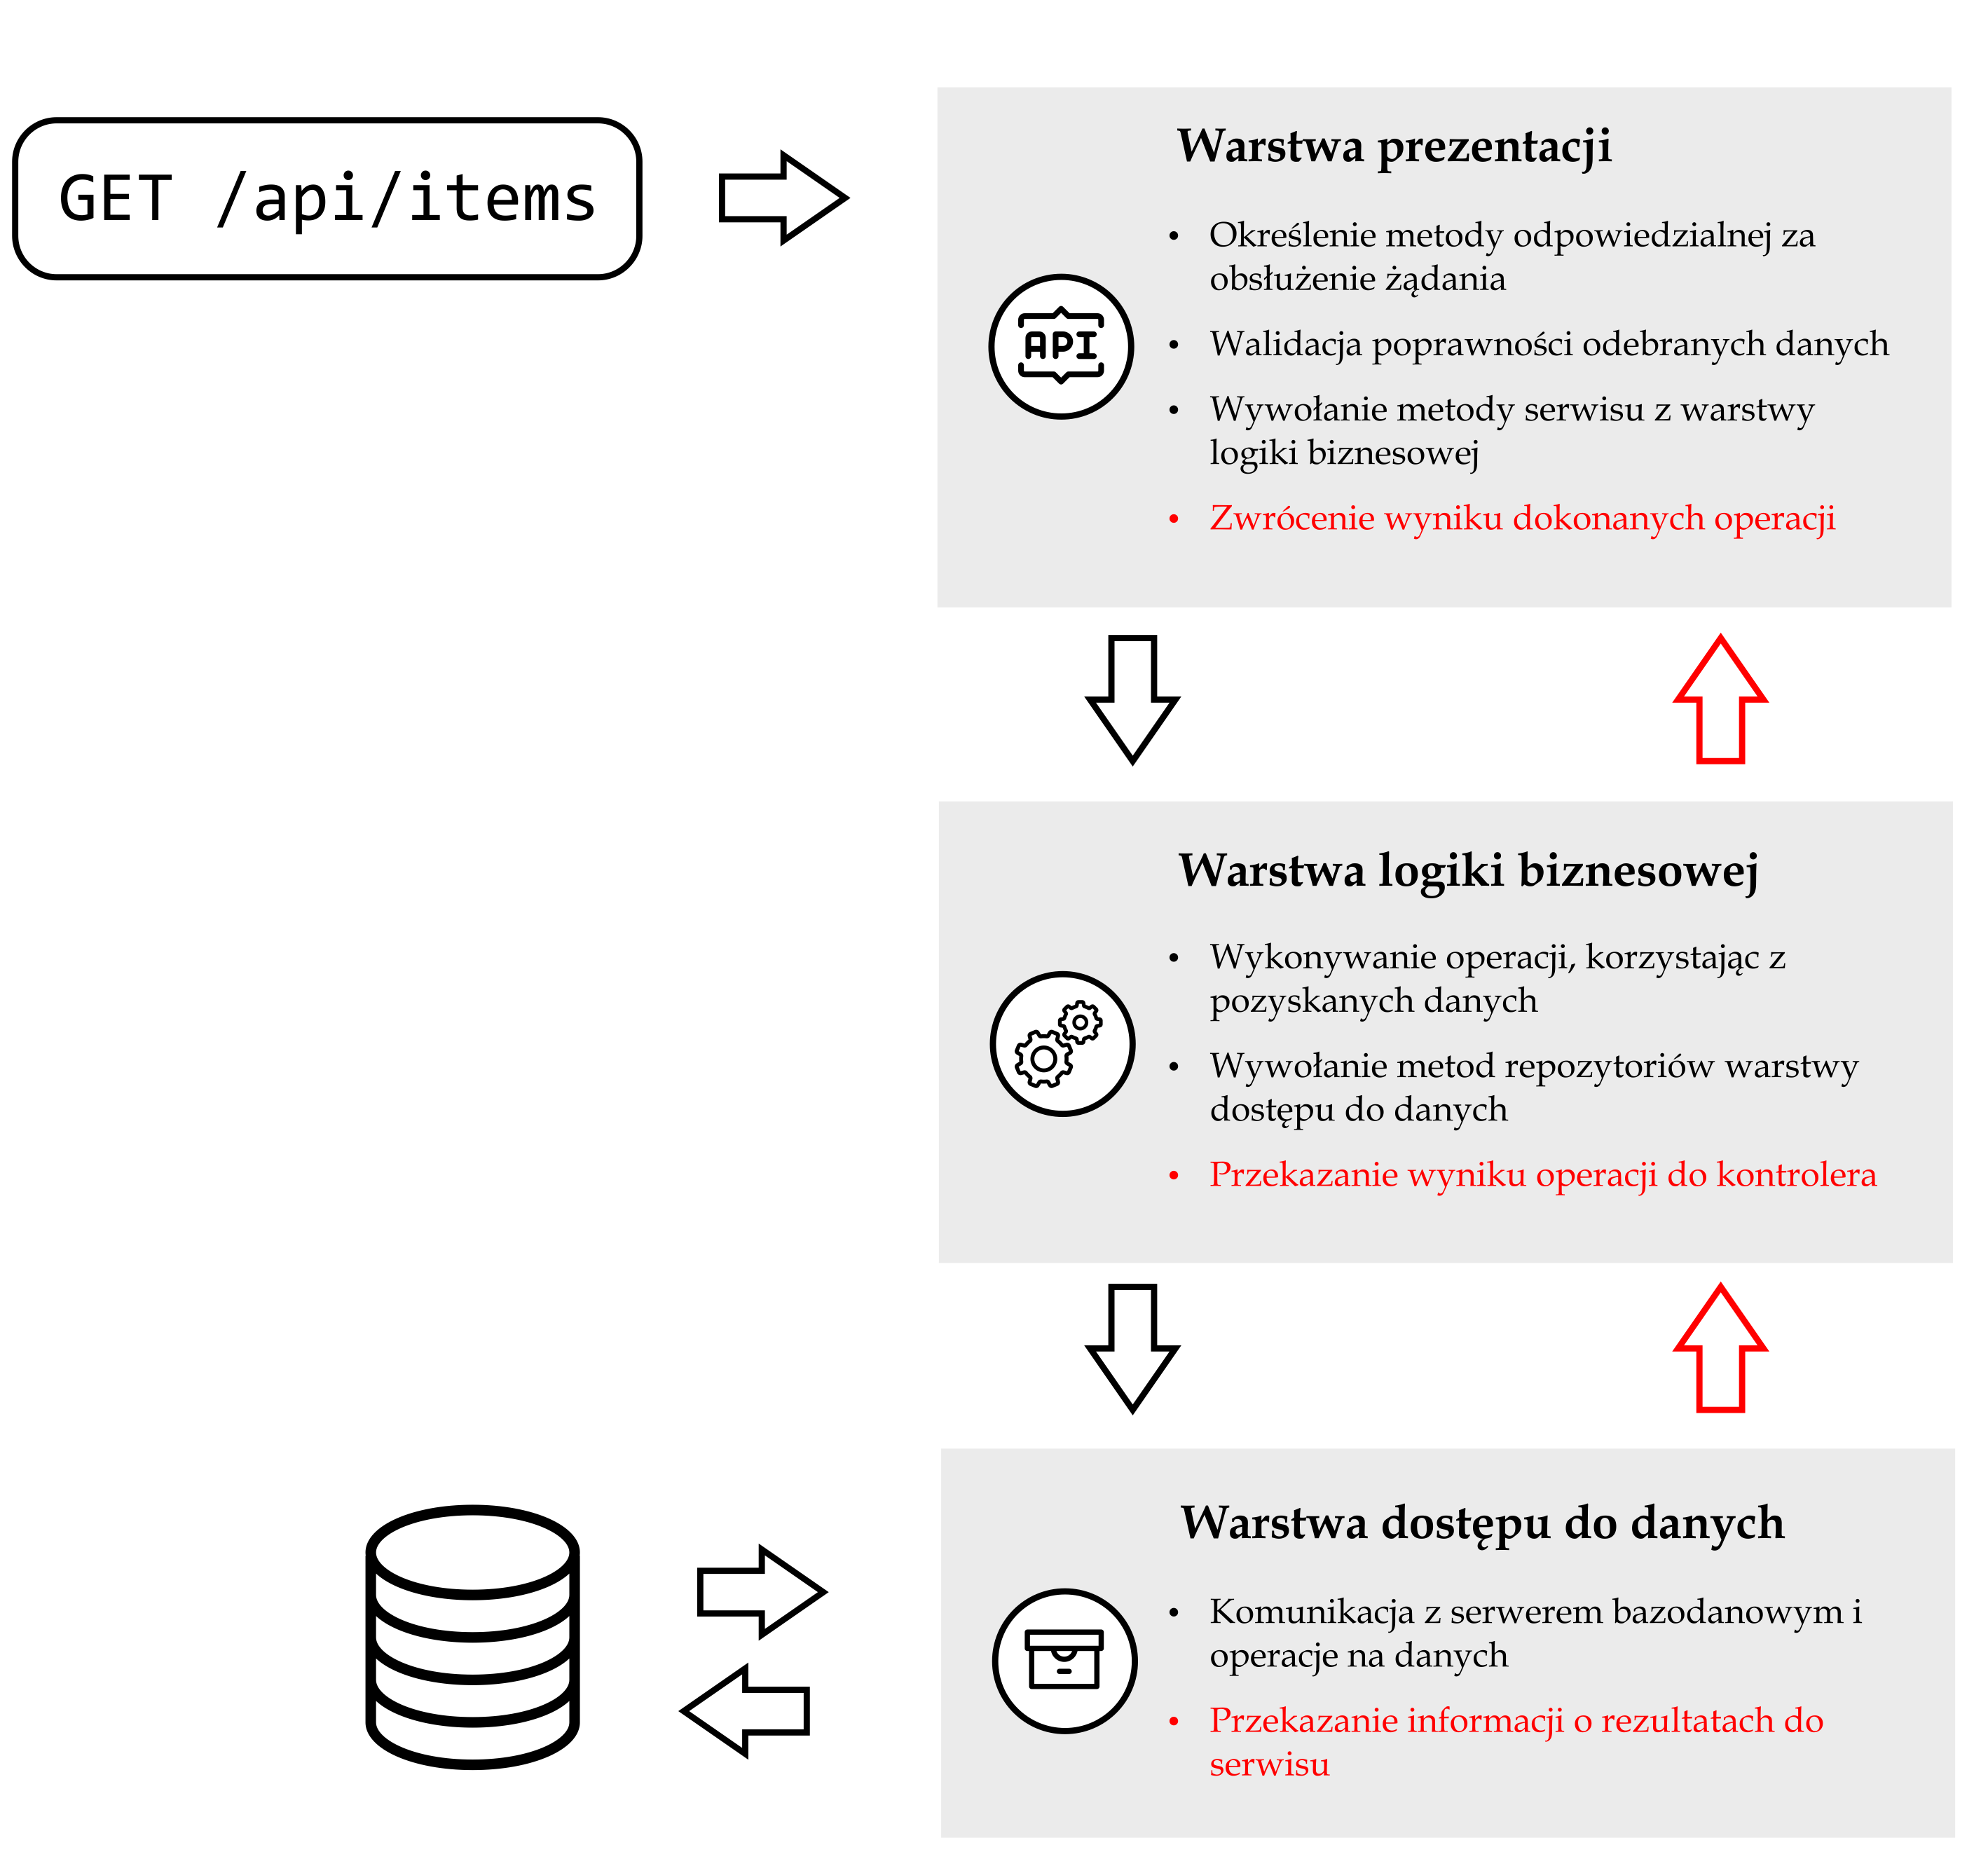
\includegraphics[width=0.9\linewidth]{rys02/architektura-api}
 \caption{Proces przetwarzania żądania wewnątrz interfejsu API}
 \label{fig:architektura-api}
\end{figure}
 
\subsection*{Konwersja obiektowo-relacyjna}
W celu uproszczenia procesu pozyskiwania oraz modyfikacji danych z zewnętrznych źródeł, a także unifikacji sposobu interakcji z nimi w ramach interfejsów programowania aplikacji powszechnie wykorzystywane jest oprogramowanie zwane mapperem obiektowo-relacyjnym (\textit{ang. Object-Relational Mapper}). Założeniem oprogramowania tego jest zdefiniowanie warstwy abstrakcji pomiędzy interfejsem programowania aplikacji a językiem programowania bądź zbiorem poleceń wykorzystywanym w ramach obsługi źródła danych.

Podstawowe składowe oprogramowania typu ORM to jednolity interfejs operacji na zbiorze danych, klasy kontekstu bazodanowego, a także metody obsługi komunikacji z bazą danych.

Dzięki wprowadzeniu jednolitego interfejsu operacji na danych niezależnie od źródła informacji z jakim komunikuje się API wydanie konkretnego polecenia do dowolnego systemu bazodanowego równoznaczne jest z każdorazowym wywołaniem funkcji o takiej samej sygnaturze. Stosując takie podejście, konstruktor interfejsu programowania aplikacji nie staje się uzależniony od źródła danych z którym pracuje. Ponadto, istnieje możliwość zamiany lub połączenia dodatkowego systemu bazodanowego, a operacja ta, nie wpływa w jakikolwiek sposób na działanie interfejsu API. Niniejsza zależność została zilustrowana na rysunku \ref{fig:orm-wyjasnienie}

\begin{figure}[ht]
 \centering
  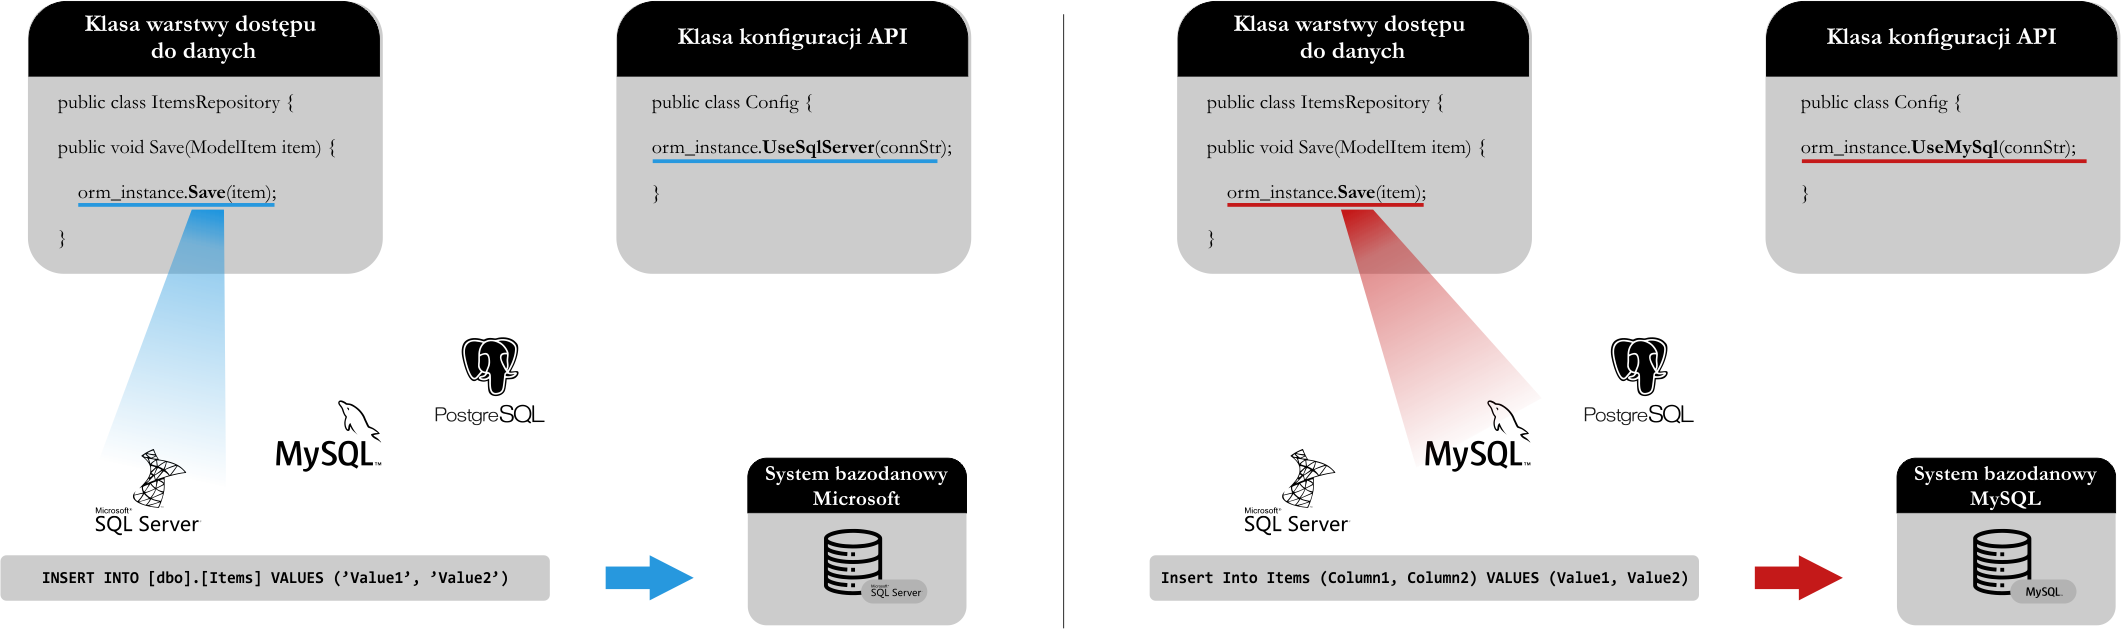
\includegraphics[width=1\linewidth]{rys02/orm-wyjasnienie}
 \caption{Zasada działania oprogramowania mappera obiektowo-relacyjnego w kontekście jednolitego interfejsu operacji na zbiorze danych}
 \label{fig:orm-wyjasnienie}
\end{figure}

Dystynktywnym elementem oprogramowania mappera obiektowo-relacyjnego jest klasa kontekstu bazodanowego. Klasa ta, jest kontenerem struktur w ramach których wyróżnić możemy zbiory elementów modelu danych, a także konfigurację poszczególnych ich właściwości. Podstawową ideą omawianej konwersji dziedziny obiektowej do domeny relacyjnej jest zdefiniowanie zbioru klas opisujących wykorzystywane zasoby, a następnie odwzorowanie ich w relacyjnym modelu danych obsługiwanym przez wybrany system bazodanowy. Klasa kontekstu pozwala na określenie, które spośród struktur danych zdefiniowanych w ramach API powinny zostać rzutowane na obiekty tabel generowanych w obrębie bazy danych. Ponadto, dla właściwości każdej z klas modelu danych zdefiniować należy konfigurację, która zostanie przetransformowana do modelu relacyjnego. W zakresie klasy kontekstu bazy danych opisywane są także relacje jakie mają zostać wygenerowane pomiędzy poszczególnymi elementami modelu.

W celu nawiązania, utrzymania, a także zakończenia komunikacji z zewnętrznym źródłem danych, oprogramowanie ORM wykorzystuje klasy zwane konektorami. Klasy te, dostarczają przejrzysty interfejs obsługi połączenia, który następnie jest opakowywany w zunifikowany interfejs dostępny bezpośrednio dla twórcy API \cite{TORRES20171}.

\subsection*{Uwierzytelnienie oraz autoryzacja}
Proces uwierzytelnienia oraz autoryzacji użytkownika odwołującego się do interfejsu programowania aplikacji przedstawić należy w trzech następujących krokach.

Pierwszym z nich jest wygenerowanie żądania odwołującego się do punktu końcowego odpowiedzialnego za obsługę uwierzytelnienia wewnątrz API. Żądanie to, musi posiadać ciało zawierające informacje poświadczające o konkretnymi użytkowniku. Najczęściej informacją tą jest nazwa użytkownika oraz hasło.

Następnie dostarczone referencje są analizowane przez mechanizmy uwierzytelniania implementowane w ramach API. W rezultacie tych operacji zwrócona zostaje pozytywna odpowiedź zawierająca token autoryzujący bądź też negatywna posiadająca w sobie informację o błędzie uwierzytelnienia klienta.

Strona kliencka może autoryzować dysponowane operacje przed interfejsem programowania aplikacji uwzględniając w ramach linii nagłówkowej żądania token uwierzytelniający. Dostarczona w ten sposób informacja pozwala na identyfikację użytkownika w ramach interfejsu API, a także na określenie przypisanego użytkownikowi poziomu uprawnień. W ramach struktury tokenu zawarta jest także informacja o jego czasie ważności. Dlatego też, procedura uwierzytelniania musi być regularnie ponawiana \cite{lakshmiraghavan2013pro}.

Na rysunku \ref{fig:uwierzytelnienie-autoryzacja} zilustrowany został proces uwierzytelnienia i autoryzacji aplikacji klienta przez interfejsem programowania aplikacji. 

\begin{figure}[ht]
 \centering
  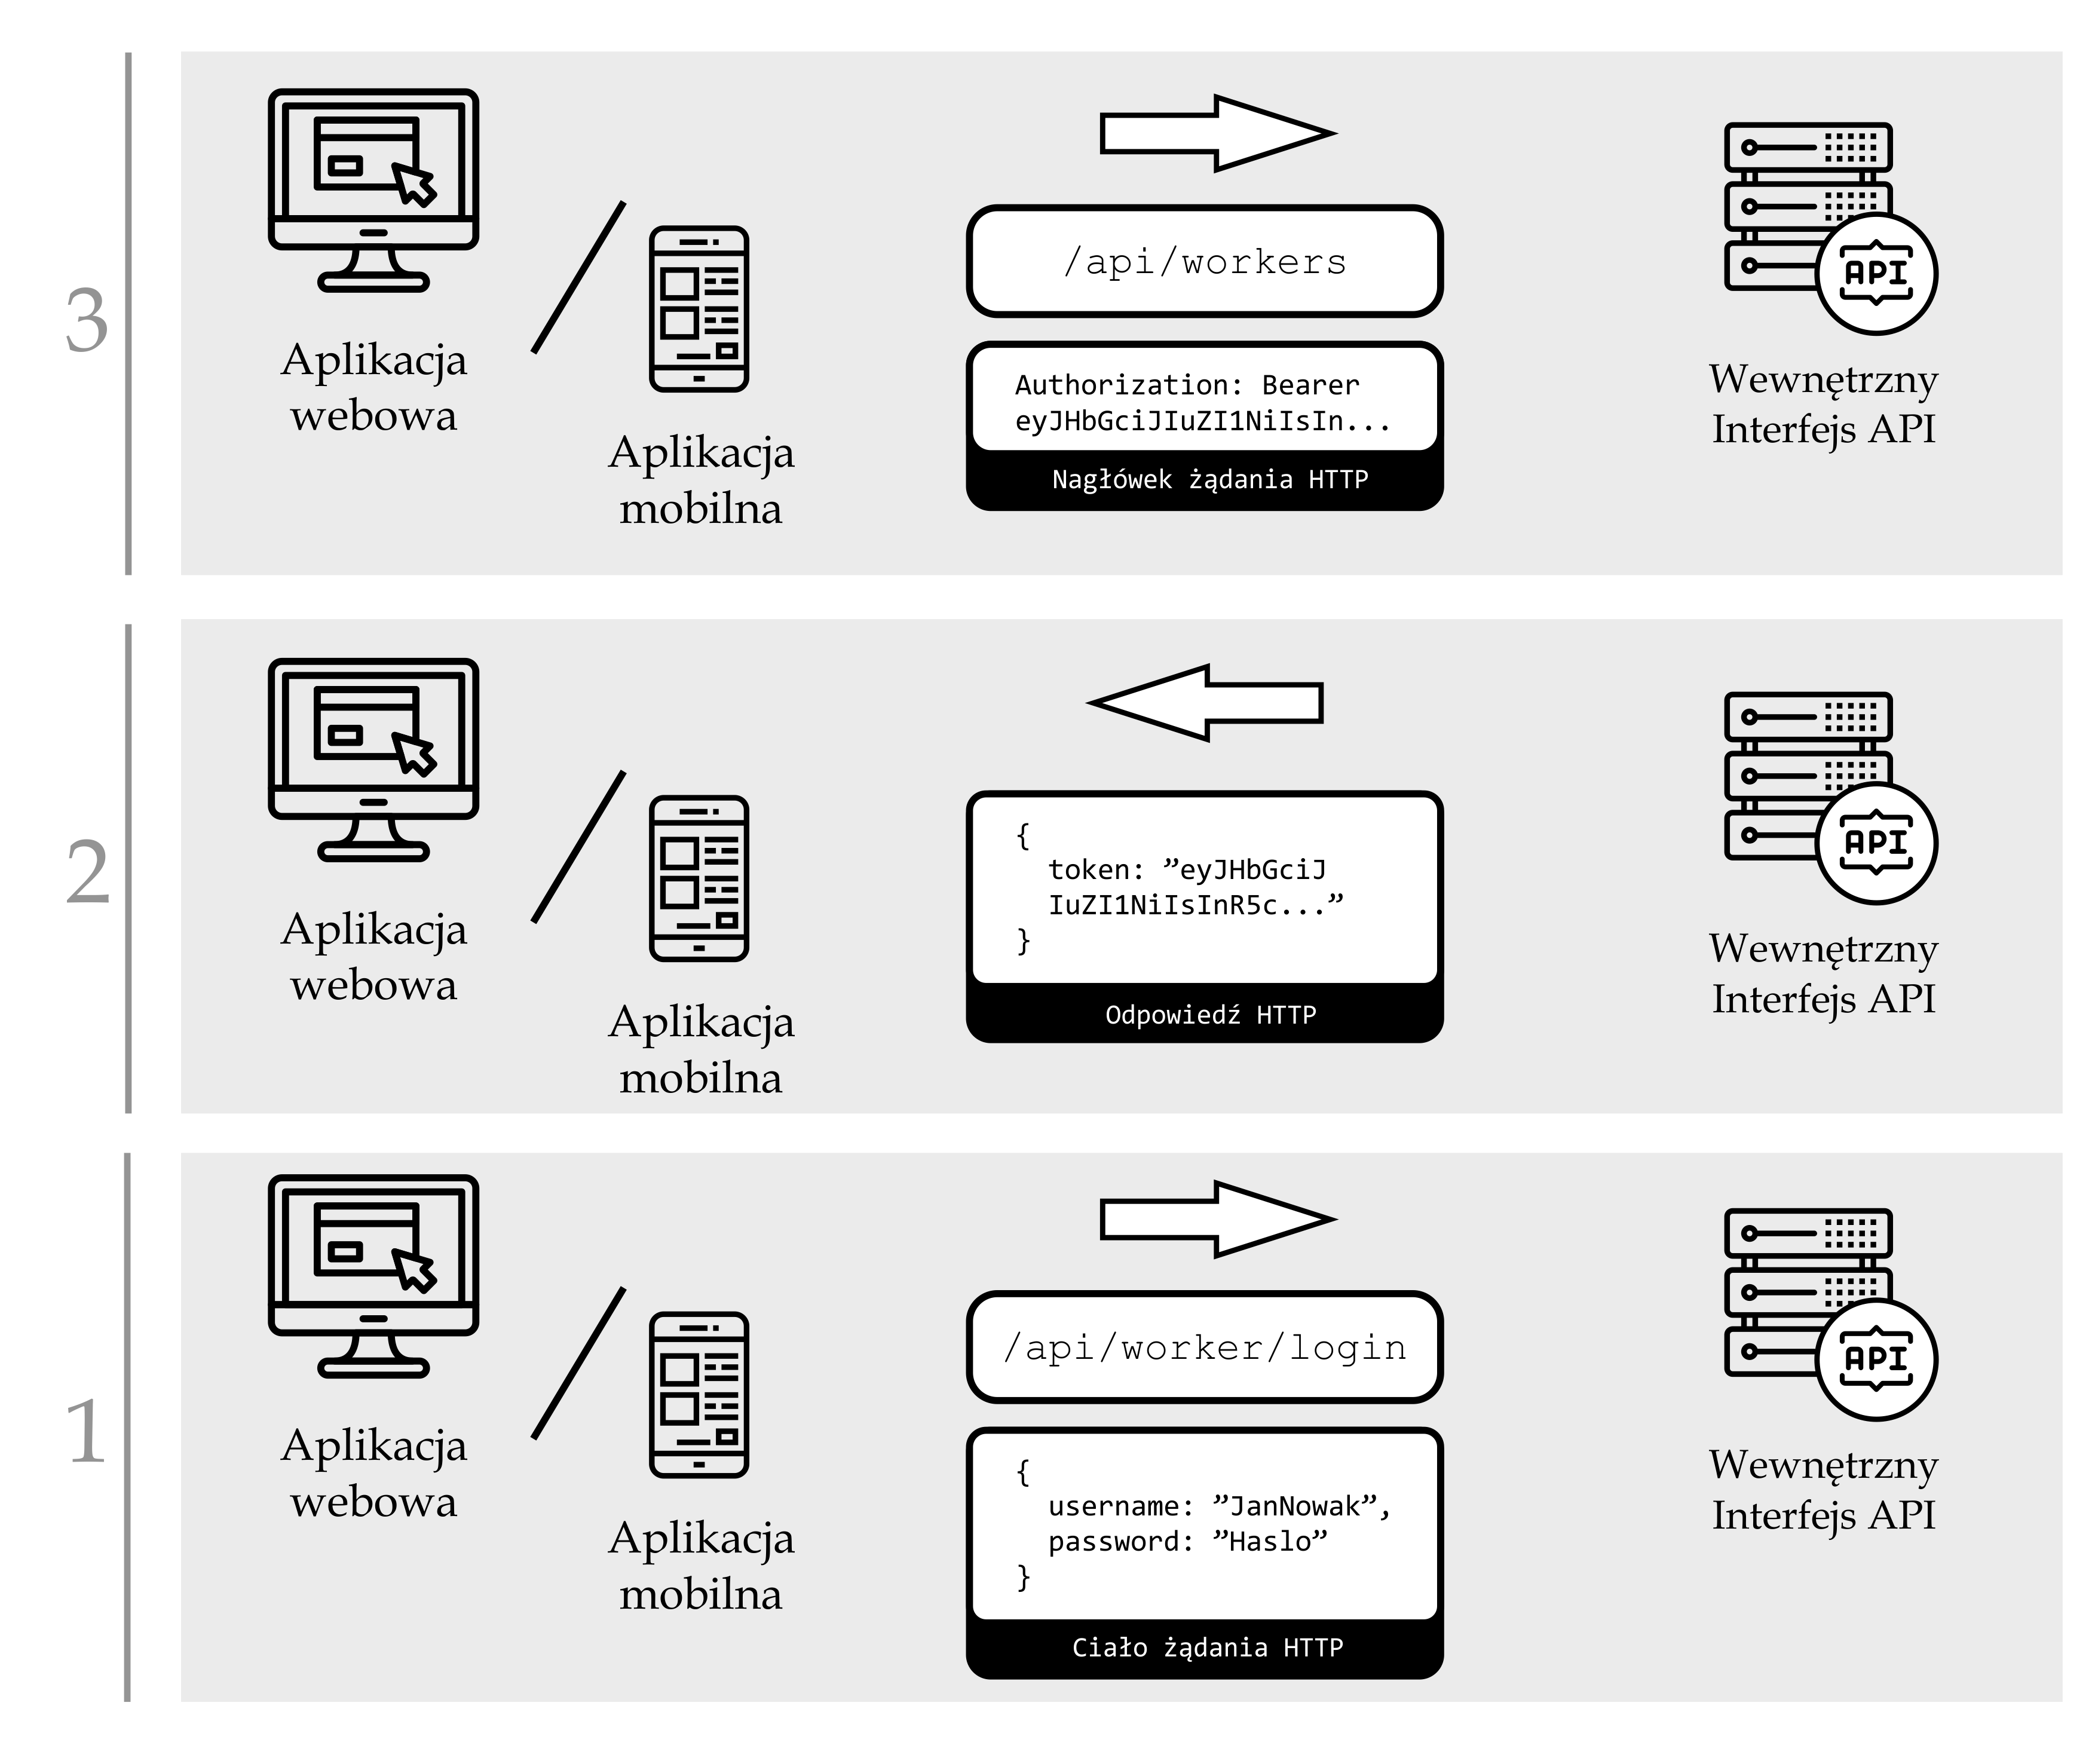
\includegraphics[width=1\linewidth]{rys02/uwierzytelnianie-autoryzacja}
 \caption{Proces uwierzytelnienia oraz autoryzacji użytkownika przed interfejsem API}
 \label{fig:uwierzytelnienie-autoryzacja}
\end{figure}


\subsection*{Separacja zapytań oraz komend w kontekście odwołań do źródeł danych}
Wraz z rosnącą liczbą żądań obsługiwanych w ramach zaawansowanych interfejsów programowania aplikacji zauważone zostało zjawisko asymetrii w kontekście typów wiadomości generowanych przez klientów. Zapytania dotyczące pozyskiwania danych z API realizowane jest z nieporównywalnie większą częstością niż operacje ich modyfikacji. Dlatego też, zdefiniowany został wzorzec projektowy dotyczący separacji zapytań oraz komend generowanych względem usługi sieciowej \textit{(ang. Command Query Responsibility Segregation)}.

Zastosowanie przedstawionego powyżej wzorca projektowego wiąże się z koniecznością budowy dwóch osobnych modeli danych. Pierwszy z nich, wykorzystywany jest w kontekście odczytu informacji. Na modelu tym, dokonywana jest najczęściej operacja optymalizacji, której celem jest redukcja rozmiaru składowych modelu, a także szybkości przetwarzania bardziej złożonych struktur będących jego częścią. Drugi z modeli danych znajduje zastosowanie w aspekcie modyfikacji określonych zasóbów. Biorąc pod uwagę standardowy sposób eksploatacji interfejsu programowania aplikacji model ten cechować się może niższą wydajnością. W zależności od specyfiki określonej usługi sieciowej optymalizowany może być albo model odczytu, albo też model zapisu. Ponadto, implementując wzorzec projektowy separacji zapytań oraz komend wykorzystać można dwa osobne zewnętrzne źródła danych przystosowane do wydajniejszego wykonywania określonego typu operacji bądź też dostosowane do obsługi większego ruchu sieciowego.   

Niewątpliwymi zaletami wynikającymi z zastosowania opisywanego wzorca projektowego są: zwiększenie efektywności operacji realizowanych z dużą częstotliwością, możliwość korzystania z osobnych źródeł danych dla operacji odczytu oraz zapisu, zachowanie zasady pojedynczej odpowiedzialności \textit{(ang. Single Responsibility Principle)} względem klas logiki biznesowej API, a także redukcja liczby wstrzykiwanych zależności \textit{(ang. Dependency Injection)} w ramach klas kontrolerów interfejsu \cite{cs7194}.

Na ilustracjach \ref{fig:standard-vs-cqrs1} oraz \ref{fig:standard-vs-cqrs2} przedstawiono kolejno schemat przetwarzania żądań wewnątrz API z uwzględnieniem wzorca CQRS, a także przy wykorzystaniu pojedynczego modelu danych.

\begin{figure}[ht]
    \centering
     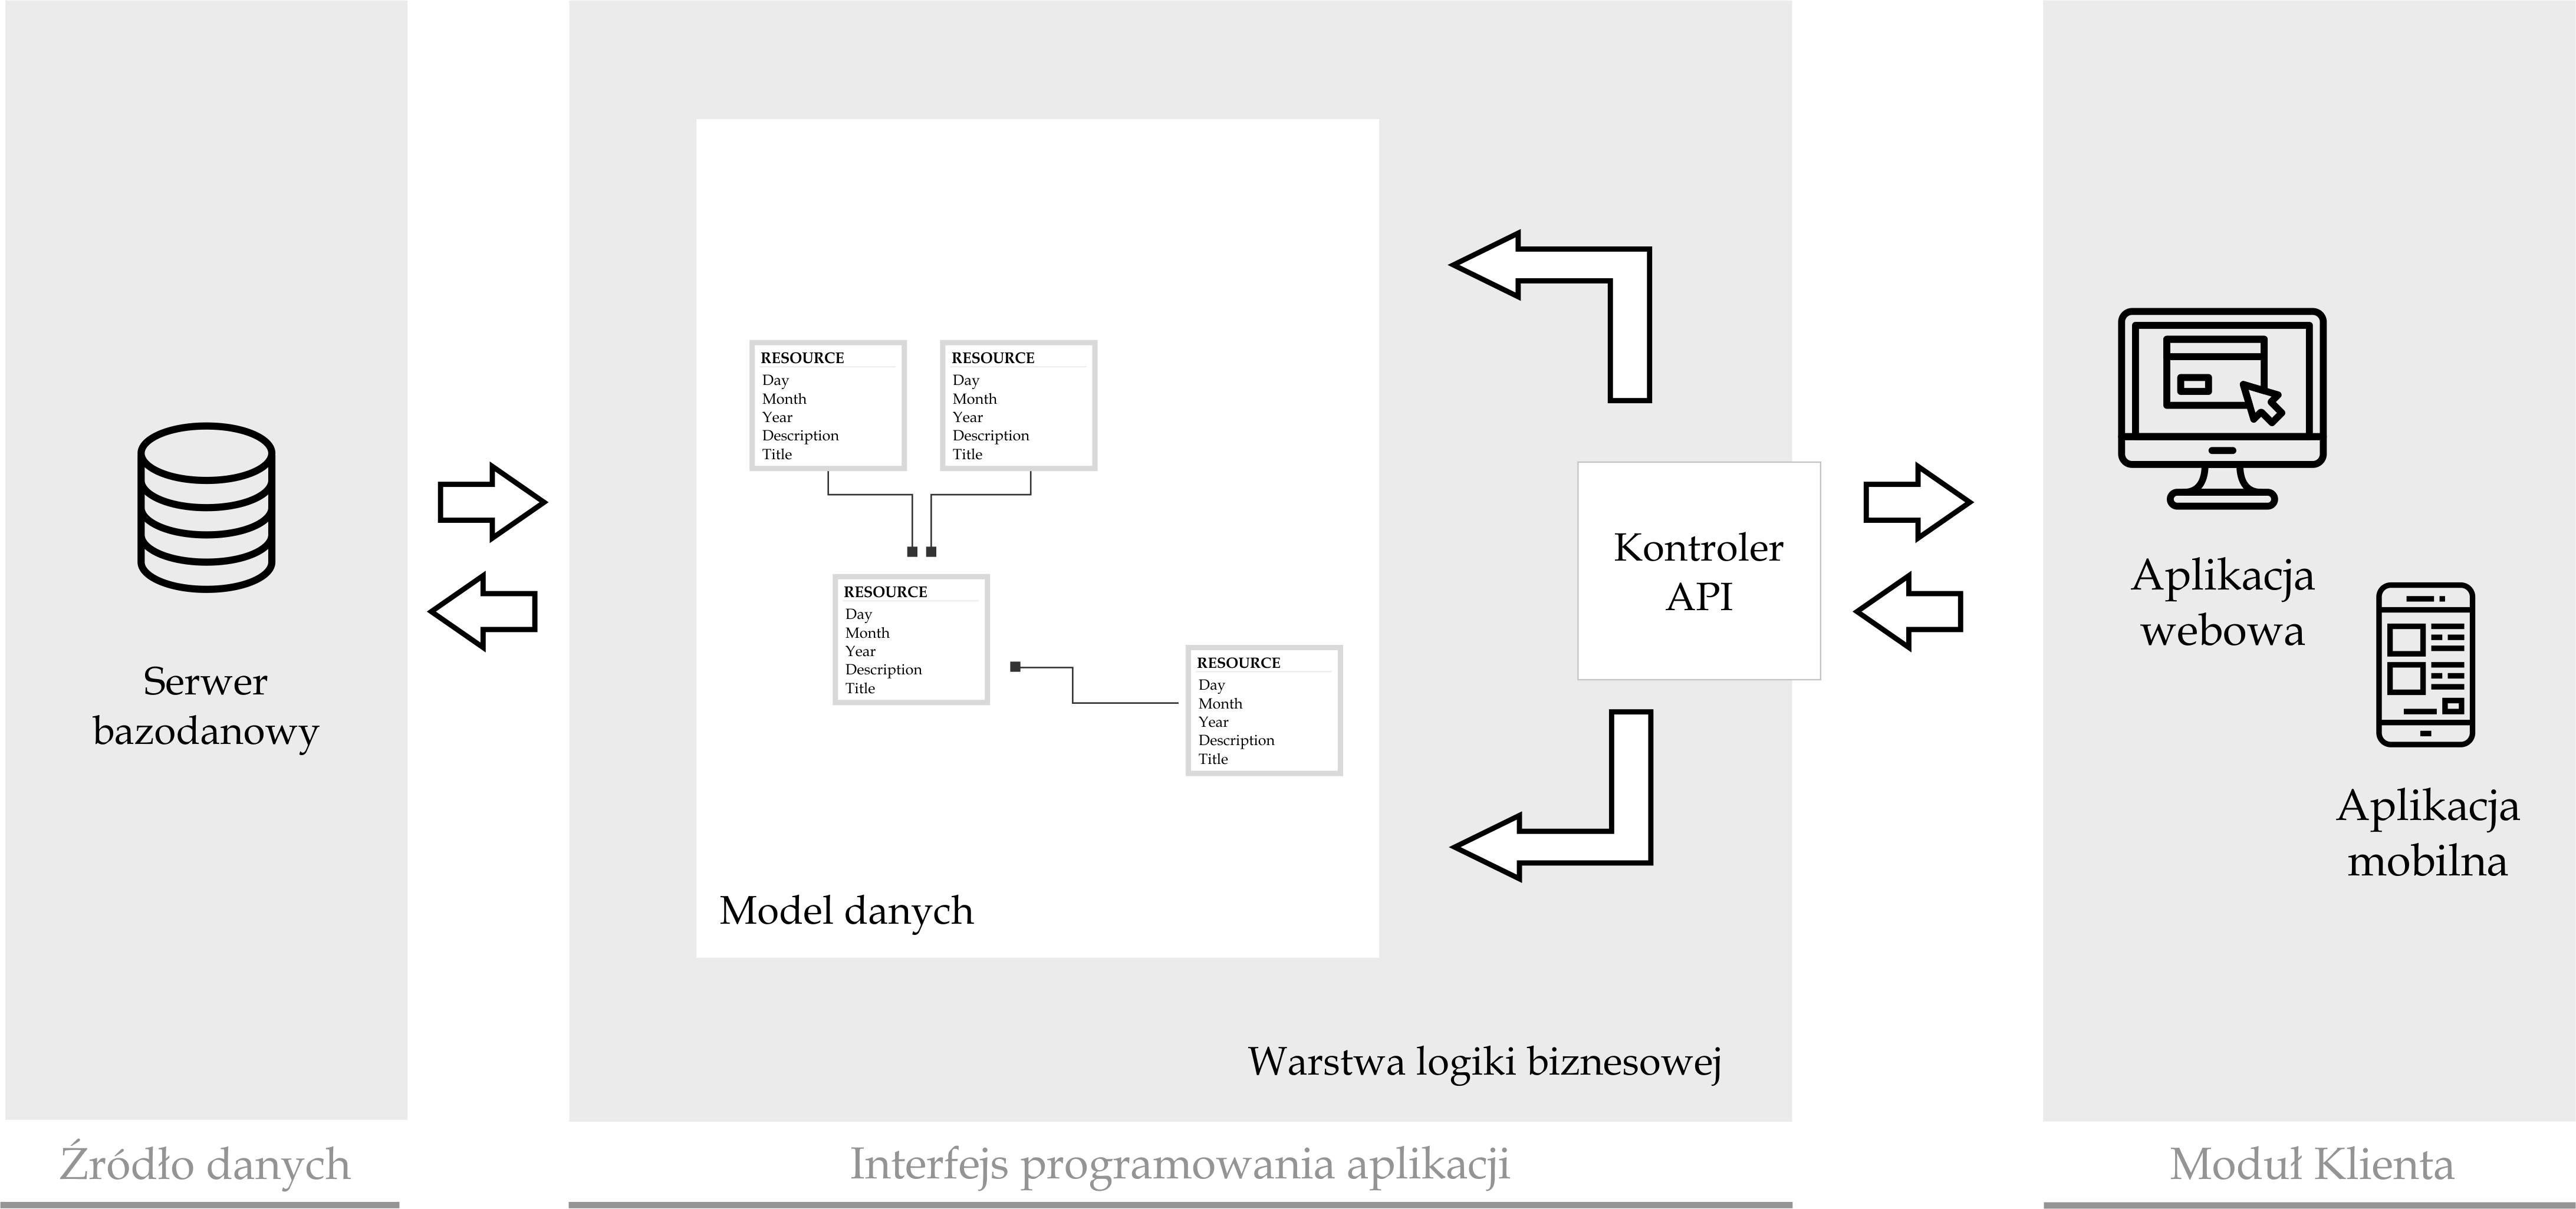
\includegraphics[width=0.9\linewidth]{rys02/standard-vs-cqrs1.png}
    \caption{Schemat przetworzenia żądania przez interfejs API dla architektury z jednym modelem danych}
    \label{fig:standard-vs-cqrs1}
   \end{figure}

   \begin{figure}[ht]
    \centering
     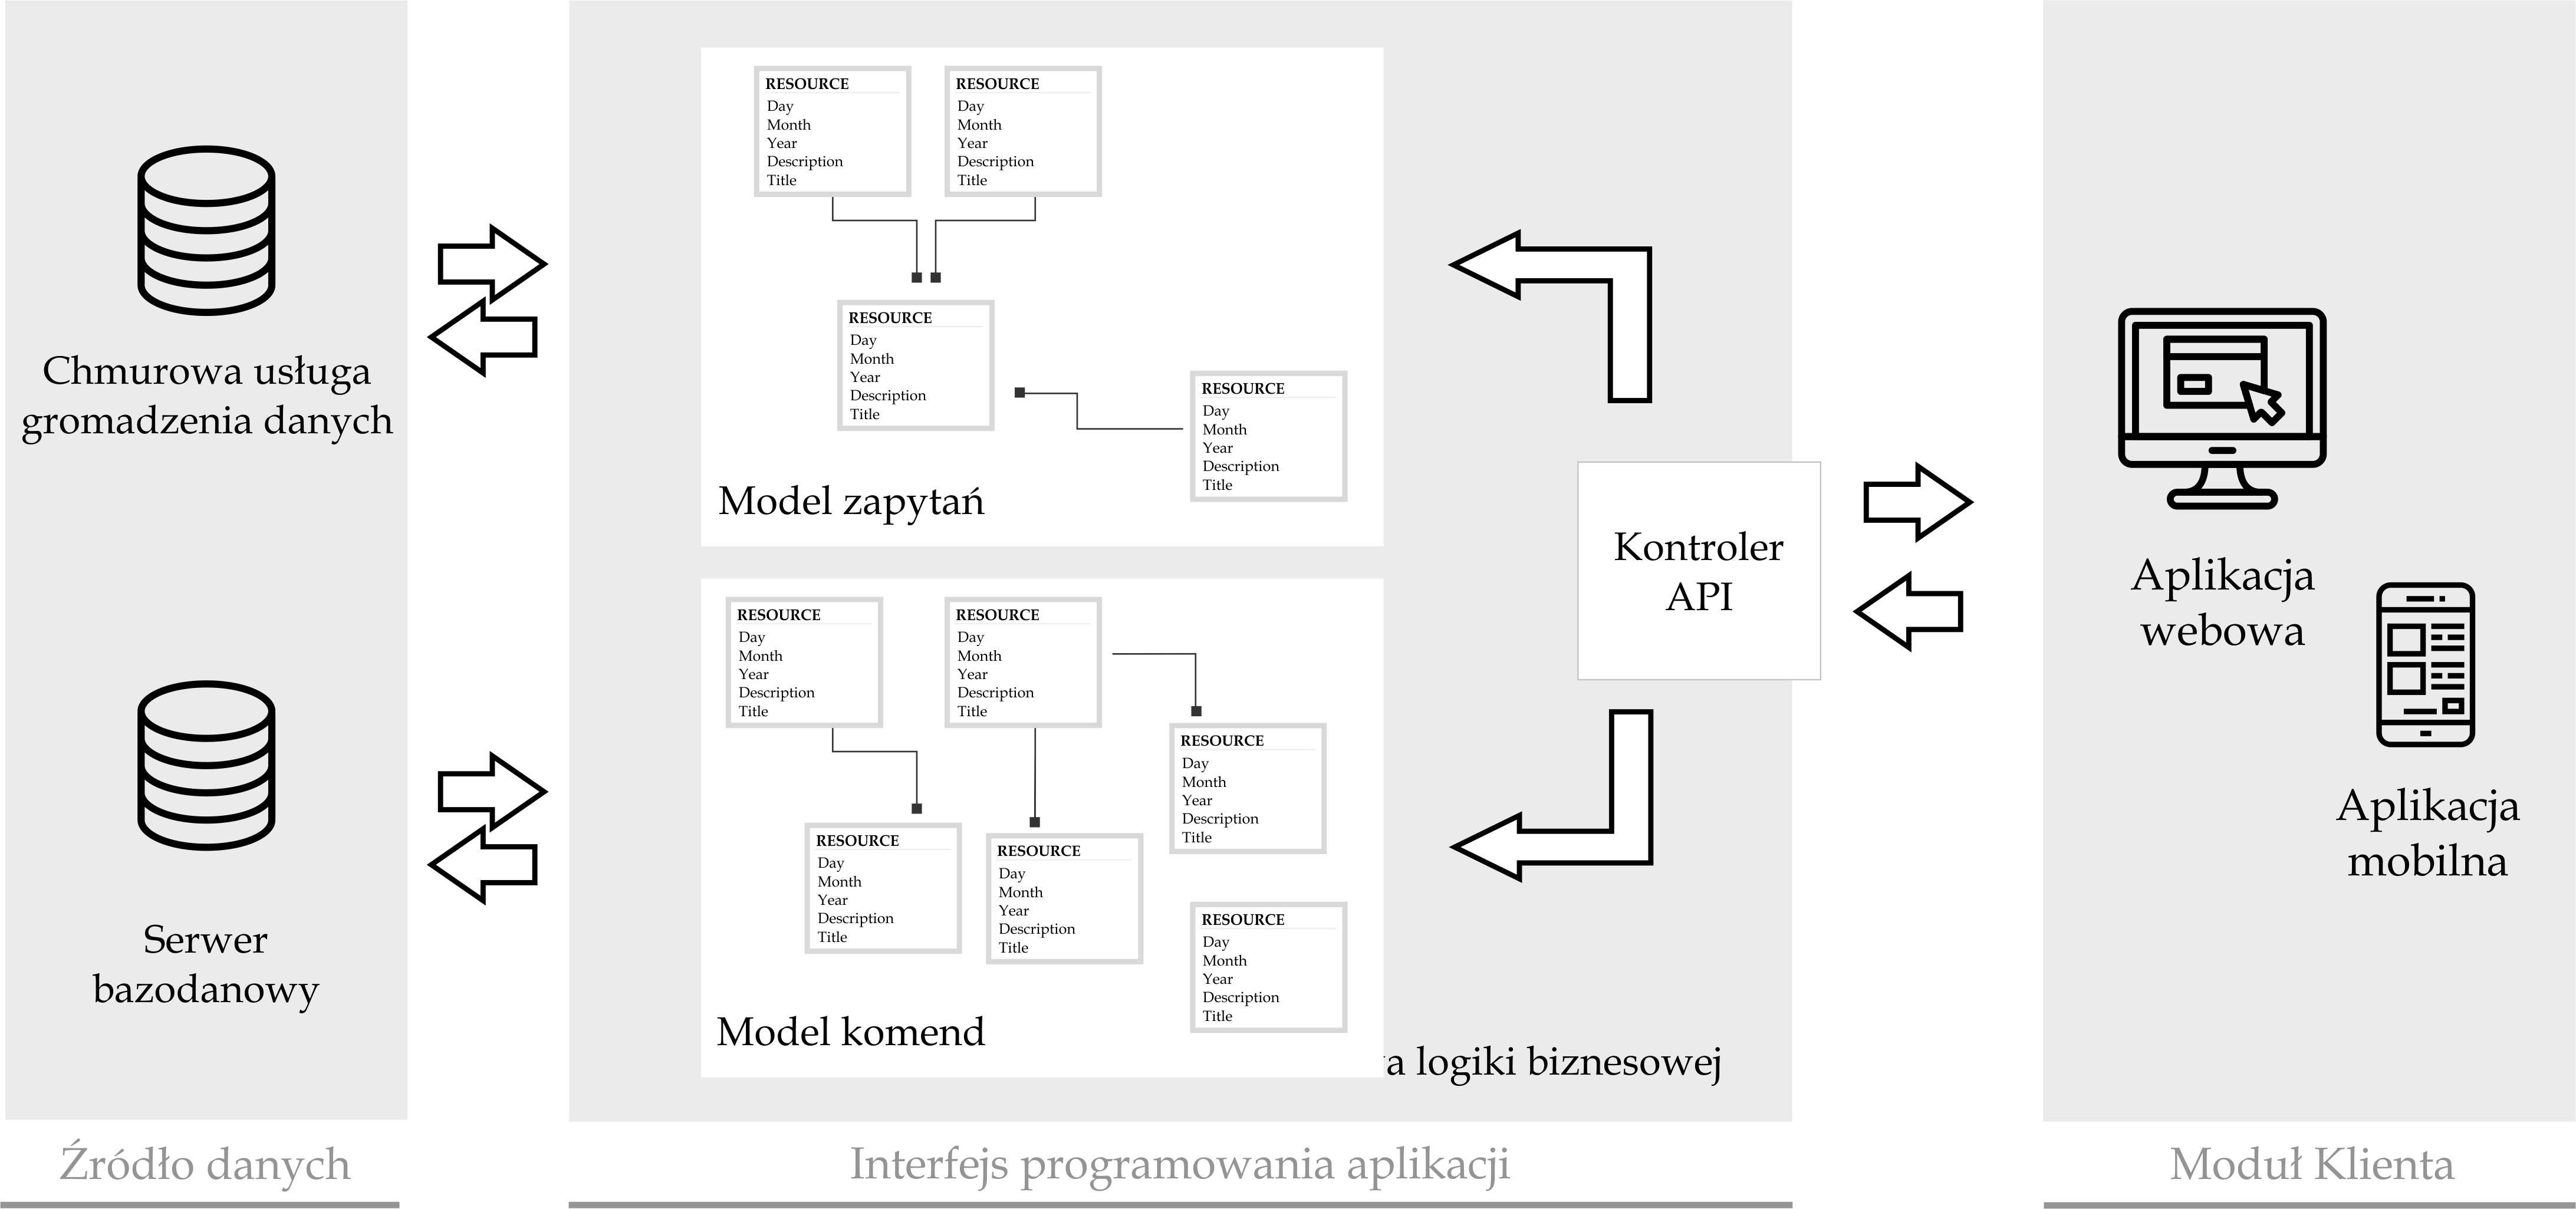
\includegraphics[width=0.9\linewidth]{rys02/standard-vs-cqrs2.png}
    \caption{Schemat przetworzenia żądania przez interfejs API dla architektury wykorzystującej wzorzec projektowy CQRS}
    \label{fig:standard-vs-cqrs2}
   \end{figure}


Odwołując się do ilustracji \ref{fig:standard-vs-cqrs2} należy zaznaczyć, że jest to jedna z możliwości implementacji wzorca CQRS uwzględniająca wykorzystanie odseparowanych źródeł danych. Architektura separacji zapytań oraz komend w kontekście żądań wysyłanych do interfejsu API może być także wprowadzona przy wykorzystaniu pojedynczego systemu bazodanowego.

\subsection*{Konwencja REST}
Niezależnie od struktury wewnętrznej omawianych usług sieciowych, współczesne interfejsy programowania aplikacji projektowane są tak aby ich zewnętrzna warstwa (tj. widziana z perspektywy aplikacji klienckiej) cechowała się jednolitą kompozycją.

Jednym z najpopularniejszych sposobów zapewnienia jednolitego interfejsu komunikacyjnego pomiędzy klientami i usługami sieciowymi przetwarzającymi informacje z wykorzystaniem protokołu HTTP jest konwencja oraz styl architektoniczny REST \textit{(ang. Representational State Transfer)}.

Konwencja ta, definiuje zbiór zasad dotyczących m.in. zachowania usługi sieciowej w kontekście przetwarzania żądania konkretnego typu, struktury i elementów odpowiedzi na określone żądanie, semantyki wykorzystywanych statusów rezultatu przetwarzania, bezstanowego charakteru komunikacji czy też syntaktyki odwołań do poszczególnych punktów końcowych.

W kontekście stopnia implementacji stylu architektonicznego REST w ramach interfejsu programowania aplikacji wprowadzić należy pojęcie modelu dojrzałości Richardsona \textit{(ang. Richardson Maturity Model)}. Pojęcie to definiuje cztery poziomy przystosowania interfejsu API do omawianej w niniejszej sekcji konwencji.

W odniesieniu do poziomu zerowego, powinnością interfejsu programowania aplikacji jest udostępnienie usług w ramach pojedynczego adresu sieciowego niezależnie od wykorzystywanych metod HTTP. Struktura żadania klienckiego w sposób jednoznaczny dostarczać ma informację na temat wykonywanego wewnątrz usługi sieciowej działania.

Zasada poziomu pierwszego odnosi się do charakterystyki interfejsu API jako usługi zorientowanej na zasoby. Niezależnie od czynności jaka ma zostać wykonana przez omawianą usługę sieciową opis tej czynności wskazywać ma na zasób którego ona dotyczy.

Reguła stanowiąca definicję poziomu trzeciego związana jest z semantyką poszczególnych typów żądań protokołu hipertekstowego. Żądanie o takim samym adresie sieciowym pełnić powinno odmienną rolę w zależności od rodzaju żądania HTTP.

Ostatnim z poziomów dojrzałości interfejsu programowania aplikacji opartego o konwencję REST jest reguła HATEOAS \textit{(ang. Hypertext As The Engine Of Application State)}. Reguła ta, definiuje interfejs API jako źródło informacji dotyczącej obsługi stanu całego systemu internetowego (tj. usługi sieciowej wraz z aplikacjami klienckimi). Klient, po uzyskaniu odpowiedzi serwera na żądanie powinien na podstawie zawartości tej odpowiedzi móc zdefiniować przyszłe czynności które wolno mu wykonać \cite{webber2010rest}.  

\section{Testowanie oprogramowania}
Aspekt badawczy niniejszej pracy związany jest z realizacją procesu ewaluacji wydajności interfejsów programowania aplikacji pod kątem wykorzystania odmiennych środowisk implementacyjnych oraz uruchomieniowych. Proces ten, jest tylko jednym z wielu elementów domeny testowania oprogramowania, której charakterystyka uwzględnia zbiór sztywno zdefiniowanych reguł cechujących się wysokim poziomem sformalizowania. W następnych sekcjach niniejszego akapitu dokonane zostało wprowadzenie dotyczące zagadnienia ewaluacji oprogramowania, nakreślone zostały zasady testowania systemów informatycznych, zdefiniono taksonomię technik testowania, a także omówiono proces przeprowadzania ewaluacji wydajności usługi sieciowej jaką jest interfejs programowania aplikacji. 
\subsection*{Wprowadzenie do zagadnienia ewaluacji oprogramowania}
Ewaluacja poszczególnych składowych tworzonego oprogramowania jest niezbędną częścią procesu budowy systemu informatycznego niezależnie od jego charakterystyki, czy też wykorzystywanej do jego budowy technologii. W rozumieniu ogólnym, proces testowania często sprowadzany jest do zbioru dwóch czynności. Czynnościami tymi są uruchamianie oprogramowania, a także eksploracja jego funkcjonalności w celu dostrzegania tych w ramach których zauważyć można niezgodność ich działania w stosunku do specyfikacji. Takie wnioskowanie jednak jest niepełne i uwzględnia ono tylko jeden z etapów składających się na cały proces testowania. Dziedzinę ewaluacji cech programów komputerowych poszerzyć należy ponadto o takie elementy jak: planowanie testów, wybór kryteriów oceny oprogramowania, nadzór oraz kontrolę realizacji badań, projektowanie przypadków testowych, czy też analizę spełnienia ustalonych kryteriów zakończenia.

Wyróżnić możemy znaczącą liczbę definicji testowania oprogramowania a każda z nich wprowadza inny poziom szczegółowości. Ponadto, wiele spośród formułowanych pojęć nawiązuje do różnych aspektów omawianego procesu. Zgodnie z jedną z najbardziej generycznych definicji wprowadzoną przez Hetzla w publikacji \cite{hetzel}, proces testowania oprogramowania określić należy jako zbiór wszystkich czynności, które nakierowane są na weryfikację atrybutów i właściwości programu, a także sprawdzenie tego czy określony system spełnia założone wymagania. Definicja ta względem wielu innych popularnych sformułowań dotyczących ewaluacji oprogramowania uwzględnia możliwość zastosowania statycznych technik testowania. Ponadto, jej autor bierze pod uwagę fakt, że w ramach procesu ewaluacji oceniany powinien być każdy z artefaktów tworzonych w ramach systemu a nie tylko i wyłącznie kod źródłowy programu.
\subsection*{Taksonomia technik testowania}
Jako jedno z podstawowych kryteriów podziału technik testowania oprogramowania wskazać należy rodzaj czynności wykonywanej przez stronę testującą, której realizacja prowadzi do uzyskania charakterystyki programu poddanego ewaluacji. Według kryterium tego wyróżnić należy statyczne oraz dynamiczne techniki testowania.

Pierwsze spośród przytoczonych metod opierają się na analizie artefaktów oprogramowania (takich jak m.in.: kod źródłowy, specyfikacja, dokumentacja, czy też lista wymagań) bez ich wykonywania. Jako praktyczne przykłady przedstawionej techniki zdefiniować należy: generowanie metryk kodu źródłowego programu, analizę przepływu sterowania, formalne dowodzenie poprawności działania, a także interpretację grafów wywołań.

Metody dynamiczne natomiast związane są z weryfikacją właściwości poszczególnych elementów systemu informatycznego w trakcie jego wykonywania. Ten rodzaj testowania nie uwzględnia formalnych struktur liczbowych jakimi są grafy przepływu sterowania czy też metryki kodu źródłowego programu. Zorientowany jest on na odbiór systemu z perspektywy korzystającego z niego klienta.

Innym z rozważanych kryteriów podziału technik testowania jest ich umiejscowienie metody względem określonego fragmentu procesu wytwórczego. W nawiązaniu do tego aspektu zdefiniować należy pojęcie poziomu testów, które jest powiązaniem sposobu ewaluacji oprogramowania z etapem jego realizacji. Istotą rozróżniania danych poziomów testów jest założenie różnorodności celów testowania, a także testowanych obiektów określanych w kontekście każdej z warstw. W odniesieniu do najbardziej popularnych systematyk poziomów testowania wyróżnić można następujące elementy:
\begin{itemize}
    \item testy jednostkowe (zwane także modułowymi lub testami komponentów),
    \item testy integracyjne,
    \item testy systemowe,
    \item testy akceptacyjne.
\end{itemize}

Pierwszy z poziomów dotyczy znajdowania niezgodności specyfikacyjnych w obrębie logicznie oddzielonych jednostek oprogramowania \textit{(ang. Software Units)}. Każda z jednostek powinna być testowana w izolacji od pozostałych elementów systemu. Ze względu na złożoność rozwiązań informatycznych, a także statystycznie wysoki współczynnik wzajemnych zależności modułowych warunek ten często nie może zostać spełniony. W takich sytuacjach, aby dostarczyć zależność do testowanej jednostki budowane są moduły zastępcze imitujące poprawne zachowanie określonego fragmentu programu \textit{(ang. Mocks)}. Omawiany poziom testowania często postrzegany jest jako jeden z etapów procesu wytwórczego, szczególnie w ramach takich technik jak rozwój oprogramowania napędzany testowaniem \textit{(ang. Test Driven Development)}.

Celem kolejnego z poziomów testowania jest weryfikacja poprawności współoddziaływania indywidualnych komponentów a także prawidłowości funkcjonowania interfejsów definiowanych pomiędzy nimi. Przykładem współdziałania jednostek oprogramowania może być współpraca interfejsu programowania aplikacji będącego systemem poddawanym analizie w ramach niniejszej pracy, a także określonego silnika bazodanowego. W zależności od liczności weryfikowanych powiązań pomiędzy poszczególnymi jednostkami oprogramowania, a także w odniesieniu do liczby samych modułów będących częścią testowanego fragmentu systemu wyróżnić możemy testy małej oraz dużej skali integracji.

Na temat testów systemowych należy mówić wtedy, gdy wszystkie z elementów rozwiązania informatycznego zostały ze sobą powiązane w sposób spójny. Celem testów realizowanych w ramach tego poziomu jest weryfikacja wysokopoziomowej funkcjonalności oprogramowania, a także wykonywanie scenariuszy ewaluacji systemu z poziomu regularnego użytkownika \textit{(ang. End-to-End testing)}.

Ostatnim z wymienionych poziomów ewaluacji są testy akceptacyjne. Przedmiotem oceny w ramach tego rodzaju testów jest gotowe rozwiązanie informatyczne w postaci komercyjnego produktu. Podmiot odpowiedzialny za realizację omawianych testów przygotowuje listę kryteriów akceptacji \textit{(ang. acceptance criteria)} a następnie na podstawie obsługi testowanego rozwiązania potwierdza lub odrzuca spełnienie każdego z nich. Celem omawianych ewaluacji nie jest znajdowanie błędów działania systemu a nabranie zaufania co do jakości jego funkcjonalnych oraz niefunkcjonalnych atrybutów.

Wykonując testy definiowane w ramach kolejnych poziomów ewaluacji weryfikowane zostają na początek funkcjonalne, a następnie niefunkcjonalne elementy testowanego systemu. Jako weryfikację elementów funkcjonalnych rozumieć należy wszystkie te czynności, które podejmowane są w ramach wszystkich wymienionych powyżej poziomów testów z wyjątkiem testów akceptacyjnych. Ewaluacja niefunkcjonalna natomiast odnosi się tylko do ostatniego spośród wyróżnionych poziomów testowania.

Podział charakteryzujący przedmiot ewaluacji względem omówionych aspektów definiuje pojęcia testów funkcjonalnych oraz niefunkcjonalnych i w kontekście niniejszej pracy jest on podziałem kluczowym.

Badania przeprowadzone w ramach tej pracy posiadają charakter testów niefunkcjonalnych, a ich wykonanie poprzedzone jest weryfikacją funkcjonalną, której poprawność traktowana jest jako wymóg.
\subsection*{Ewaluacja wydajności interfejsów programowania aplikacji}
Zgodnie z teorią przedstawioną w sekcji \ref{sec:api-teoria} niniejszej pracy interfejs programowania aplikacji postrzegać można jako deterministyczny system wejściowo-wyjściowy o charakterze dyskretnym. Takie podejście, w znaczący sposób ułatwia proces ewaluacji wydajności interfejsów API.

Definiowanie interfejsu API jako systemu pobudzanego pojedynczym wejściem, a także generującego pojedynczą wartość wyjściową, pozwala na wykorzystanie sposobu oceny wydajności zwanego testem czarnoskrzynkowym \textit{(ang. Black-box testing)}. W ramach tego rodzaju testu, określone kryterium ewaluacji wyliczane jest jako różnica wartości pomiaru na wyjściu systemu, względem tej, której kalkulacja nastąpiła na jego wejściu. Taki rodzaj testu, umożliwia wyliczenie metryki wydajności, bez konieczności przygotowywania systemu do przeprowadzenia procesu testowania.

Podstawowym kryterium oceny wydajności interfejsu programowania aplikacji jest czas odpowiedzi na żądanie. Metrykę tę, określić należy jako czas od momentu wygenerowania żądania przez stronę klienta, do chwili uzyskania przez niego odpowiedzi. Zauważyć należy również zależność czasu odpowiedzi na żądanie, zarówno od rozmiaru żądania jak i wielkości jego odpowiedzi. Ponadto, czynnikiem wpływającym na uzyskany rezultat pomiaru jest niewątpliwie przepustowość łącza sieciowego pomiędzy klientem a serwerem.

Aby rezultaty uzyskane w ramach oceny wydajności API mogły zostać postrzegane jako rzetelne, omówione powyżej czynniki muszą cechować się statyczną charakterystyką, bądź też zostać całkowicie wyeliminowane z procesu testowego. W ramach niniejszej pracy, rozmiar odpowiedzi generowanej przez interfejsy programowania aplikacji jest stały niezależnie od zastosowanej technologii, a także środowiska uruchomieniowego. Wynika to z zastosowania pojedynczego i ustrukturyzowanego modelu danych, który jest identyczny, niezależnie od API. W odniesieniu do zmienności prędkości łącza internetowego, aspekt ten został wyeliminowany poprzez przeprowadzanie testów w obrębie lokalnej sieci komputerowej, a także umiejscowienie interfejsów oraz systemów bazodanowych w ramach tej właśnie sieci.

Kolejnym z kryteriów oceny wydajności, uwzględnianym w ramach procesu testowania usług sieciowych jest poprawność uzyskanej odpowiedzi w odniesieniu do liczby klientów, równolegle generujących żądania. Kryterium to, charakteryzuje się silną korelacją z czasem odpowiedzi na pojedyncze zapytanie.

Uwzględniając oba opisane powyżej parametry, podstawowy schemat scenariusza badawczego dotyczącego ewaluacji wydajności API składa się z następujących testów:
\begin{itemize}
    \item testy linii bazowej -- pojedynczy klient generuje żadania w kierunku API w celu zdefiniowania średniego czasu odpowiedzi usługi w standardowych warunkach jej działania. W ramach niniejszej pracy, podczas wykonywania omawianego testu, zdefiniowane zostaną ponadto wartości współczynników satysfakcji, toleracji oraz frustracji, będące składowymi wskaźnika jakości APDEX. Wartości te, stanowią uogólnioną ocenę wydajności i posłużą jako punkt odniesienia dla kolejnych testów.
    \item testy obciążeniowe -- uwzględniana zostaje zmienna liczba klientów generujących żądania, w kontekście której ustalane są średnie czasu odpowiedzi na żądanie, a także dokonywane zostaje odniesienie uzyskanego rezultatu do współczynników zdefiniowanych uprzednio w ramach miary APDEX.
    \item testy przeciążające -- liczba klientów generujących żądanie zostaje dobrana w taki sposób, aby doprowadzić do obciążenia testowanej usługi, niepozwalającego na poprawne funkcjonowanie interfejsu programowania aplikacji. Ewaluacja ta, ma na celu znalezienie punktu krytycznego w kontekście działania testowanego oprogramowania.
\end{itemize}

Poza czarnoskrzynkowymi testami wydajności, cechującymi się omówioną powyżej strkturą, przeprowadzone mogą zostać ewaluacje efektywności działania poszczególnych fragmentów usługi sieciowej, w ramach których interfejs programowania aplikacji postrzegać należy w odmienny sposób, aniżeli jako system wejściowo-wyjściowy.

Przykładem oceny wydajności określonego fragmentu interfejsu programowania aplikacji może być ewaluacja modułu realizacji zaawansowanych operacji obliczeniowych, dostępnego z poziomu punktu końcowego API. W takim przypadku, oprogramowanie musi zostać dostosowane do przeprowadzenia procedury testowej, a metryka wydajności - powiązana z postępem realizacji obliczeń.
\section{Wykorzystywane narzędzia i technologie}
Zarówno w trakcie procesu implementacji badanych interfejsów programowania aplikacji, jak i procedurze przeprowadzenia badań pod kontem ich wydajności, wykorzystano obszerny zbiór sprawdzonych i powszechnie stosowanych rozwiązań technologicznych. W ramach niniejszej sekcji, opisane zostanie każde z nich.

\subsection*{C\#}
C\# jest wieloparadygmatowym, a także nowoczesnym językiem programowania ogólnego przeznaczenia, charakteryzującym się bezpieczeństwem i niezawodnością w aspekcie typowania struktur danych. Pierwsza z wersji tego języka, stworzona została przez Andersa Hejlsberga w roku 1998. Od tamtej chwili, do momentu napisania niniejszej pracy, upublicznionych zostało 9 kolejnych,  stabilnych wydań projektu C\#. Każda z następnych wersji omawianego języka programowania wprowadzała zarówno usprawnienia w kontekście ekosystemu budowy i kompilacji programów źródłowych, jak i wzbogacała interfejs bibliotek funkcyjnych o kluczowe z punktu widzenia doświadczonego programisty rozwiązania. Do rozwiązań tych, zaliczyć należy między innymi: mechanizmy programowania współbieżnego, typy anonimowe, operatory zmiennych typów niezdefiniowanych, obsługę referencji, typy generyczne, czy też wyrażenia lambda. 

W ramach niniejszej pracy, język C\# wykorzystany został do implementacji jednego z dwóch zbiorów interfejsów programowania aplikacji. Ze względu na zastosowanie rozwiązań z zakresu przetwarzania współbieżnego (tj. operacji asynchronicznych oraz wielowątkowych) udostępnianych przez omawiany język programowania, interfejsy API realizowane w tej technologii mogą obsługiwać w sposób równoległy żądania pochodzące od wielu klientów, a także utrzymywać sekwencyjny charakter przetwarzanych procedur niezależnie od czasu ich wykonywania. Należy także zwrócić uwagę na mechanizm wewnętrznych usprawnień wydajnościowych implementowany w ramach kompilatora i uruchamiany w momencie tłumaczenia kodu języka do tzw. języka pośredniego \textit{(ang. Intermediate Language)}. Dzięki zastosowaniu przedstawionego mechanizmu, operacje zdefiniowane przez programistę mogą być modyfikowane w procesie kompilacji, tak aby nie wpłynąć na zaimplementowaną funkcjonalność, zwiększając jednocześnie wydajność generowanego programu \cite{hejlsberg2003c}.
\subsection*{.NET Core}
.NET Core postrzegać należy jako środowisko budowy, kompilacji oraz wykonywania rozwiązań implementowanych w języku C\#. Przedstawiana technologia stanowi podzbiór bibliotek, dzięki którym programista jest w stanie budować systemy różnorodnego przeznaczenia, a także uruchamiać je w wielu wspieranych środowiskach programowych. W przeciwieństwie do technologii .NET Framework będącej poprzednikiem .NET Core, aplikacje tworzone na bazie omawianej biblioteki mogą być wydawane nie tylko na system operacyjny Windows, ale także na systemy Linux oraz MacOS.

W ramach omawianego środowiska wykorzystywany zostaje komponent języka C\# zwany biblioteką standardową \textit{(ang. .NET Standard Library)}. Biblioteka ta jest wspólna dla wielu środowisk uruchomieniowych, a zawarte w niej funkcjonalności, traktować należy jako metody ogólnego przeznaczenia.

Ponadto, środowisko .NET Core, w ramach procesu budowy i kompilacji rozwiązania nawiązuje komunikację z komponentem wspólnej infrastruktury \textit{(ang. Common Infrastructure)}. Komponent ten, podobnie jak biblioteka standardowa, współdzielony jest przez wiele środowisk wykonawczych. W kontekście wspólnej infrastruktury, wspomnieć należy o wspólnej specyfikacji języka \textit{(ang. CLS -- Common Language Specification)}, wspólnym systemie typów \textit{(ang. CTS -- Common Type System)}, a także środowisku uruchomieniowym wspólnego języka \textit{(ang. CLR -- Common Language Runtime)}. Wykorzystanie między innymi tych trzech elementów, pozwala na budowę systemu dostępnego na wielu platformach \cite{troelsen2017pro}.

W kontekście realizowanej pracy, technologia .NET Core użyta została jako środowisko uruchomieniowe dla interfejsów programowania aplikacji tworzonych w języku C\#. W obrębie technologii tej, poza przedstawionymi powyżej komponentami, wyróżnić możemy natywną bibliotekę ASP.NET Core, stanowiącą zbiór metod przydatnych w procesie definiowania internetowych usług sieciowych oraz aplikacji webowych. Dzięki zastosowaniu ASP.NET Core operacje takie jak, między innymi: obsługa definicji kontrolerów API, zarządzanie stanem ciała żądania oraz jego rzutowaniem na określony typ danych, czy też implementacja mechanizmów uwierzytelniania i autoryzacji klienta, wykonane mogą zostać na wysokim poziomie abstrakcji z jednoczesnym zapewnieniem należytego poziomu ich wydajności.
\subsection*{Entity Framework Core}
Entity Framework Core stanowi narzędzie stworzone przez firmę Microsoft, którego zastosowaniem jest mapowanie obiektowo-relacyjne realizowane w kontekście usług internetowych tworzonych z wykorzystaniem języka C\# oraz uruchamianych na platformie .NET Core. Przedstawiana biblioteka zapewnia programiście zorientowany obiektowo interfejs, za pomocą którego może on uzyskać dostęp do danych, a także je definiować oraz przetwarzać. Zbiory obiektów mogą być składowane zarówno w relacyjnych jak i niereleacyjnych bazach danych. Niniejsza biblioteka, podobnie do środowiska uruchomieniowego .NET Core, jest rozwiązaniem wieloplatformowym i może być wykorzystywana przy budowie systemów internetowych wdrażanych na systemach Windows, Linux oraz MacOS.

Zastosowanie biblioteki mapera obiektowo-relacyjnego jaką jest Entity Framework Core umożliwia zastosowanie podejścia zorientowanego na kod źródłowy w kontekście aplikacji komunikujących się i wykorzystujących zewnętrzne zbiory danych \textit{(ang. Code-First Approach)}. Podejście to, polega na definiowaniu w ramach kodu źródłowego zbioru klas modelu danych, które będą następnie przekształcane do postaci tabel określonego systemu bazodanowego. Przedstawiona operacja przekształcenia wykonywana jest bezpośrednio za pomocą mechanizmów mapera obiektowo-relacyjnego. 

Niezaprzeczalną zaletę wykorzystania biblioteki ORM jaką jest Entity Framework Core stanowi możliwość operowania na jednolitym interfejsie realizacji operacji na danych, niezależnie od obsługiwanego systemu bazodanowego. Oznacza to, że w momencie zmiany dostawcy zewnętrznego źródła danych, zawartość kodu źródłowego programu nie musi podlegać modyfikacji \cite{smith2021entity}.
\subsection*{MediatR}
MediatR to otwartoźródłowa biblioteka języka C\#, z wykorzystaniem której zaimplementowany może zostać wzorzec projektowy, dotyczący separacji odpowiedzialności za obsługę zapytań oraz komend przetwarzanych przez usługę sieciową. Kluczowym elementem biblioteki MediatR jest para generycznych interfejsów, za pomocą których implementowana jest obsługa zarówno żądań jak i zapytań dotyczących danych. Interfejsami tymi są kolejno: \textit{IRequest} -- struktura programistyczna implementowana przez klasy definiujące zawartość ciała żądania lub komendy, a także powiązany z nią \textit{IRequestHandler}, który jest konkretyzowany przez klasę definicji metody obsługi żądania bądź operacji na danych. 

Ponadto, należy również podkreślić znaczenie metody \textit{Send} dostępnej w ramach głównego API pakietu MediatR. Dzięki niej, wywołana może zostać procedura obsługi określonego żądania lub operacji, z dowolnego miejsca kodu źródłowego interfejsu programowania aplikacji \cite{mediatr}.
\subsection*{JavaScript}
JavaScript to wielofunkcyjny oraz wieloplatformowy skryptowy język programowania cechujący się wysokim poziomem abstrakcji. Najbardziej popularnym przeznaczeniem omawianego języka jest budowa systemów internetowych, a także mobilnych. Historyczną rolą technologii JavaScript było udostępnianie programiście funkcjonalności umożliwiających określanie różnorodnych sposobów interakcji pomiędzy użytkownikiem serwisu internetowego, a jego statycznymi elementami. Podstawowym środowiskiem wykonania oraz interpretacji omawianego języka była uwcześnie przeglądarka internetowa. Wraz z pojawieniem się serwerowego środowiska uruchomieniowego NodeJS, przeznaczonego dla języka JavaScript, popularność omawianej technologii wzrosła w gwałtownym tempie. Zmianie uległo również główne przeznaczenie technologii, która od tej pory stała się pełnoprawnym językiem programowania, stosowanym w kontekście budowy zarówno systemów internetowych, rozwiązań mobilnych, jak i programów desktopowych.

Język JavaScript uznać należy za technologię charakteryzującą się typowaniem słabym oraz dynamicznym. W związku z zastosowaniem przez twórców rozwiązania takiego właśnie podejścia, tworzone kody programów narażone są na występowanie zjawisk niezgodności typów, a także niejawnej koercji. Ponadto, w kontekście mechanizmów omawianego języka, realizacja operacji przetwarzania współbieżnego oraz wykonania metod asynchronicznych, zależna jest w całkowitym stopniu od rozwiązań implementacyjnych poczynionych w ramach środowiska uruchomieniowego. Oznacza to, że przetwarzanie i wykonywanie operacji wielowątkowych może cechować się zróżnicowaną wydajnością, w zależności od konkretnego interpretera języka.  

Niewątpliwymi zaletami technologii JavaScript są: składnia cechująca się niskim poziomem złożoności poleceń, możliwość dowolnego wykorzystywania wielu spośród wspieranych paradygmatów programowania, modułowość i skalowalność implementowanych rozwiązań, a także elastyczność w kontekście operowania na wykorzystywanych strukturach danych \cite{jensen2009type}.

W ramach niniejszej pracy, język JavaScript zastosowany został w celu implementacji jednego z dwóch zbiorów badanych interfejsów programowania aplikacji. Tworzone w omawianym języku API, wykonywane będą w środowisku uruchomieniowym NodeJS.
\subsection*{TypeScript}
TypeScript stanowi statycznie typowany nadzbiór języka JavaScript. Określenie to, oznacza że omawiana technologia nie jest stricte językiem programowania, a tylko określoną grupą instrukcji oraz procedur, które włączyć można do języka JavaScript, po to, aby zapewnić w jego kontekście statyczny sposób typowania danych. Technologia TypeScript nie może być wykorzystywana samodzielnie, a środowisko wykonawcze JavaScript jest wymagane w celu uruchomienia skompilowanego modułu, definiowanego zgodnie ze składnią omawianego języka.

Kluczowym elementem przedstawianej technologii jest transpilator języka TypeScript o nazwie tsc \textit{(ang. TypeScript Compiler)}. Program ten, uruchamiany jest tuż przed rozpoczęciem procedury interepretacji kodu JavaScript i przekształca on metody odpowiedzialne za obsługę typów danych, do struktur dostępnych w ramach standardowej implementacji języka. Dlatego też, z punktu widzenia środowiska uruchomieniowego, dostępne programistom mechanizmy definicji typów czy interfejsów, nie są znane.

Celem zastosowania omawianego nadzbioru językowego jest możliwość kontroli zgodności definiowanych obiektów programistycznych pod kątem ich wewnętrznej struktury. Ponadto, wykorzystanie TypeScript umożliwia weryfikację faktu nieumyślnego odwołania się do struktury typu nieokreślonego, jeszcze przed rozpoczęciem procesu interpretacji kodu \cite{bierman2014understanding}.
\subsection*{NodeJS}
NodeJS jest środowiskiem uruchomieniowym języka JavaScript zbudowanym w oparciu o otwartoźródłowy silnik interpretacji kodu Chrome V8. Dzięki zastosowaniu omawianego środowiska uruchomieniowego, kod źródłowy języka JavaScript może być wykonywany poza ekosystemem przeglądarki internetowej. Rozwój niniejszej technologii, doprowadził do diametralnej zmiany w obszarze zastosowania języka JavaScript, a także gwałtownego wzrostu jego popularności w kontekście budowy systemów internetowych.

Podobnie do rozwiązania Microsoft .NET Core, platforma NodeJS składa się nie tylko ze środowiska uruchomieniowego, ale także ze zbioru bibliotek oraz narzędzi linii komend. Aplikacje budowane na bazie omawianej technologii cechują się zastosowaniem architektury sterowanej zdarzeniami \textit{(ang. Event-driven architecture)}, która ponadto wzbogacana jest (dzięki wykorzystaniu mechanizmu pętli) o możliwość obsługi operacji asynchronicznych. Co więcej, rozwiązania definiowane na podstawie środowiska NodeJS posiadają budowę modułową, co przyczynia się do zwiększenia ich zdolności w kontekście skalowania systemów.

Należy również uwypuklić generyczność charakterystyki środowiska NodeJS. Nie jest ono przeznaczone stricte do definiowania i wdrażania usług sieciowych, a wykorzystywane jest do uruchamiania dowolnego kodu języka JavaScript, jaki może zostać stworzony za pomocą jego składni. Dlatego też, aby dostarczać mechanizmy dotyczące specyficznych funkcjonalności, ekosystem NodeJS może być rozbudowywany poprzez otwartoźródłowe moduły. Liczność modułów tych, a także popularność ich wykorzystania stanowi niewątpliwie o sile omawianej technologii \cite{casciaro2020node}.
\subsection*{ExpressJS}
ExpressJS stanowi bibliotekę środowiska NodeJS, dostarczającą zbiór metod pozwalających na budowę webowych interfejsów programowania aplikacji w tym właśnie środowisku. Pakiet ExpressJS cechuje się minimalizmem w kontekście złożoności udostępnianych programiście operacji, elastycznością dotyczącą współpracy z zewnętrznymi pakietami, a także wysoką wydajnością działania tworzonych aplikacji, poprzez eliminację złożonych funkcjonalności przetwarzania zasobów w obrębie żądania.

Koncepcja przetwarzania zasobu uzyskanego od klienta w ramach ExpressJS sprowadza się do potokowej obsługi dostarczonego wejścia, przez kolejne funkcje pośredniczące \textit{(ang. Middleware functions)}. Ostatnia z funkcji ma za zadanie zwrócić odpowiedź wygenerowaną na podstawie operacji wykonywanych przez wszystkie poprzednie metody. Ciałem funkcji pośredniczącej może być zarówno kod źródłowy zdefiniowany przez programistę, jak i ten dostarczony poprzez referencję do zewnętrznego pakietu. Do każdej z metod przekazywane są parametry żądania, odpowiedzi, a także referencji do następnego middleware. Dzięki uruchomieniu napisanej w taki sposób aplikacji w środowisku NodeJS, poszczególne funkcje pośredniczące mogą być realizowane asynchronicznie \cite{mardan2014express}.
\subsection*{Prisma}
Prisma ORM to narzędzie pełniące rolę mapera obiektowo-relacyjnego wykorzystywanego w kontekście implementowania interfejsów programowania aplikacji w języku JavaScript. Dystynktywną cechą omawianego narzędzia jest prostota definiowania rzutowanego modelu danych. W przypadku pakietu Prisma, cała struktura modelu danych opisywana jest w ramach jednego pliku zwanego plikiem schematu. W pliku tym, określane zostają zarówno właściwości poszczególnych encji modelu, jak i relacje które między nimi występują.

Analogicznie do narzędzia Entity Framework Core, Prisma ORM wspiera zarówno relacyjne jak i nierelacyjne systemy bazodanowe. Ponadto, zauważyć należy kompatybilność omawianego narzędzia z omawianą wyżej technologią TypeScript \cite{prisma}.
\subsection*{Mongoose}
Biblioteka Mongoose stanowi narzędzie rzutowania obiektowego modelu danych definiowanego w ramach kodu programu, do postaci obiektowej nierelacyjnej bazy danych MongoDB. Technologii tej nie należy nazywać maperem obiektowo-relacyjnym, gdyż wykonywane przez nią operacje synchronizują struktury danych, które zarówno po stronie kodu, jak i po stronie źródła danych cechują się obiektową naturą.

Połączenie interfejsu programowania aplikacji z nierelacyjnym źródłem danych obsługiwanym poprzez bibliotekę Mongoose, prowadzić może do zwiększenia efektywności oraz zmniejszenia czasu wykonania operacji na danych. Jednakże, w związku z naturą przechowywanych informacji, a także brakiem uwzględniania w ich strukturze metadefinicji, zastosowanie omawianego mechanizmu może również prowadzić do braku spójności źródła danych, a także niemożliwości zastosowania usprawnień wydajnościowych w kontekście bazy danych \cite{holmes2013mongoose}.  
\subsection*{Apache JMeter}
Narzędzie Apache JMeter to otwartoźródłowe oprogramowanie stworzone w języku Java. Program ten, wykorzystywany jest przeprowadzania ewaluacji wydajności oprogramowania sieciowego opierającego swoje działanie o protokoły HTTP oraz FTP. Testy efektywności działania usług mogą zostać przeprowadzane w trybie lokalnym (tj. z wykorzystaniem jednego hosta wysyłającego żądania do określonej usługi sieciowej), jak i w trybie rozproszonym (tj. budowana zostaje hierarchia hostów będących generatorami żądań). W ramach niniejszej pracy, zastosowany został drugi z przedstawionych trybów ewaluacji.

Działanie oprogramowania Apache JMeter sprowadza się do wykonywania pętli testowej, w ramach określonych grup wątków. Pętla testowa symuluje sekwencyjne generowanie żądań w kierunku serwera, z uwzględnieniem stałej wartości opóźnienia pomiędzy wysyłanymi pakietami. Grupa wątków natomiast, określa współbieżny charakter testów obciążenia usługi sieciowej i może być utożsamiana zarówno z konkretnymi wątkami procesora lokalnego hosta, jak i z oddzielnie pracującymi generatorami żądań w trybie rozproszonym.

W celu zdefiniowania testu wydajności w ramach Apache JMeter, zbudowany powinien zostać plan testowy. Jest to podstawowa jednostka wyróżniana w ramach niniejszego oprogramowania i skupia ona w sobie między innymi komponenty grup wątków, próbników \textit{(ang. Samplers)}, a także elementów nasłuchujących na odpowiedź usługi \textit{(ang. Listeners)}. Zarówno próbniki, jak i elementy nasłuchujące mogą być powielane w ramach planu testowego, a także indywidualnie konfigurowane, w zależności od specyfiki usługi sieciowej.

Oprogramowanie Apache JMeter obsługiwać można zarówno z poziomu narzędzia linii komend, jak i udostępnionego graficznego interfejsu użytkownika \cite{halili2008apache}. 
\section{Przegląd literatury}
W niniejszym rozdziale przedstawione zostaną pozycje literaturowe, do których odnosić się będzie opisywana praca dyplomowa. Pozycje te, podzielone zostały na oddzielne grupy, związane z określoną tematyką.

Na początku, przedstawiona zostanie literatura powiązana z aspektem budowy interfejsów programowania aplikacji oraz będąca wprowadzeniem do wykorzystywanych technologii. Następnie, opisane zostaną pozycje traktujące o wydajności interfejsów API, a także o analizie działania powszechnie dostępnych serwisów internetowych opartych o metodologię REST. Kolejne prace, skupiać się będą na tematyce testowania usług sieciowych, teorii testowania, a także konfiguracji narzędzi dla testów rozproszonych. W następnej kolejności, wspomniane zostaną prace naukowe oraz dokumenty standaryzacyjne dotyczące sposobu działania protokołu przesyłania danych hipertekstowych. Ostatnią grupą pozycji literaturowych będą prace referencyjne dotyczące badań wydajności systemów internetowych.

Pozycja \cite{troelsen2017pro} stanowi wprowadzenie do zaawansowanych konceptów języka C\#, a także dostarcza informacji związanych z wykorzystaniem tego języka w środowiskach uruchomieniowych .NET oraz .NET Core. W początkowych rozdziałach przedstawiono sposób budowy, kompilacji oraz wykonywania programu w środowisku .NET. Kolejno opisana została struktura bazowych aplikacji uruchamianych w tym właśnie środowisku i tworzonych za pomocą języka C\#. Ostatnim elementem wprowadzenia do opisywanej technologii było przedstawienie struktur języka w kontekście obiektowego paradygmatu programowania.    W następnych sekcjach literatury, w sposób wyczerpujący poruszono tematykę bardziej zaawansowanych aspektów programowania w języku C\#, którymi są między innymi: kolekcje i typy generyczne, delegaty i wyrażenia lambda, czy też cykl życia obiektu w pamięci programu. Ważnym tematem, poruszonym w ramach tej książki jest struktura oraz zasada działania środowiska .net core, będącego podstawowym elementem interfejsów programowania aplikacji tworzonych w języku C\#.

Analogiczną do przedstawionej powyżej pozycji literaturowej, dotyczącą jednak technologii NodeJS oraz języka JavaScript jest \cite{casciaro2020node}. W ramach tej pracy zawarto obszerne wprowadzenie do platformy NodeJS uwzględniające ponadto kwestie obsługi operacji wejścia/wyjścia, wykonywania natywnego kodu JS, czy też przetwarzania operacji przez silnik NodeJS oraz bibliotekę libuv. Znaczna część pracy, obejmuje przedstawienie zaawansowanych wzorców projektowych, których głównym przeznaczeniem jest obsługa zdarzeń oraz operacji asynchronicznych. Wspomniane zostały także rozwiązania dotyczące skalowalności aplikacji z wykorzystaniem mechanizmów kolejkowania wiadomości.

Niezależnie od wykorzystywanej technologii, interfejsy programowania aplikacji, które zostały zbudowane na potrzeby tej pracy dyplomowej, oparte są o styl architektoniczny RESTful. Styl ten, jest pewnym zbiorem zasad projektowania usług sieciowych, określającym zarówno aspekty sposobu komunikacji klienta z usługą sieciową, jak i techniczne wymagania dotyczące przetwarzania żądań. Dobre praktyki, które uwzględnia metodologia REST, zawarte zostały w pozycji literaturowej \cite{subramanian2019hands}. Autorzy tego dokumentu, na wstępie dokonują porównania architektury zorientowanej na zasoby, będącej podstawą konwencji REST, z popularną uprzednio architekturą zorientowaną na usługi. Następnie, przedstawiane są najlepsze praktyki, cele oraz reguły REST dotyczące projektowania interfejsu programowania aplikacji. Co więcej, w omawianej książce zawarte zostały także podstawowe oraz zaawansowane wzorce projektowania API, uwzględniające aspekty bezstanowości, paginacji, osiągalności, a także identyfikacji zasobów interfejsu. Końcowe rozdziały książki, wprowadzają w kwestie testowania oraz bezpieczeństwa REST API, omawiają technikę kompozycji usług RESTful, a także przedstawiają rozwiązania (biblioteki oraz języki programowania) pozwalające na tworzenie interfejsów API zgodnych z metodologią REST.

Podstawowym celem działania interfejsu programowania aplikacji jest dostarczenie danych do konsumenta, bądź też ich manipulacja zgodnie z jego żądaniem. Aby operować na danych, interfejs API musi komunikować się ze źródłem danych, którym najczęściej jest serwer bazodanowy. W celu dostarczenia metod komunikacji pomiędzy API a źródłem danych, które jednocześnie są niezależne od wykorzystywanego źródła, a także pozwalają na zarządzanie danymi z poziomu struktur języka, stworzone zostały biblioteki zwane maperami obiektowo-relacyjnymi (ang. Object-Relational Mappers). Dla API napisanego w języku C\# podstawowym rozwiązaniem ORM jest biblioteka Entity Framework Core, która przedstawiona została w pozycji \cite{smith2021entity}. Pozycja ta, uwzględnia zarówno opis działania najczęściej wykorzystywanych metod służących do manipulacji danymi, jak i rolę klasy kontekstu bazodanowego w procesie tłumaczenia operacji programistycznych na polecenia bazodanowe. Ponadto, dowiedzieć możemy się jak przetwarzać zaawansowane typy danych (takie jak np. DateTime), czy też w jaki sposób wykorzystywać zapytania LINQ do budowania kwerend.

Dla interfejsu programowania aplikacji napisanego w języku JavaScript i uruchamianego w środowisku NodeJS, w przeciwieństwie do platformy .NET, zastosować możemy zdecydowanie większą liczbę bibliotek pełniących rolę maperów obiektowo-relacyjnych. Biblioteki te, zostały opisane w pozycjach \cite{bojinov2018restful} i \cite{laksono2018testing}. Pozycja \cite{bojinov2018restful} pełni rolę całościowego wprowadzenia do tematyki tworzenia interfejsów API, korzystając z platformy NodeJS, frameworka ExpressJS oraz nierelacyjnej bazy danych MongoDB. Rodział piąty tej pracy, traktujący o wykorzystaniu baz danych NoSQL, przybliża tematykę jednego z najczęściej wykorzystywanych maperów obiektowo-relacyjnych dla Node czyli mongoose. Przedstawiono tutaj sposób zestawienia połączenia z serwerem bazodanowym, tworzenia encji modelu, przekształcanego następnie na struktury bazy danych, a także wykonywania operacji dostępu do danych i ich modyfikacji. W pracy \cite{laksono2018testing} natomiast, porównano nierelacyjne podejście do składowania danych typu geograficznego z podejściem relacyjnym, wykorzystując w tym przypadku biblioteki mongoose i sequelize. Oba mapery obiektowo relacyjne zostały użyte w ramach interfejsu API wykorzystującego technologie NodeJS/ExpressJS. Celem opisywanej pracy było przedstawienie różnic w czasach odpowiedzi API na uzyskane żądanie, dla różnej liczby danych geolokalizacyjnych, uwzględniając zastosowanie relacyjnych i nierelacyjnych baz danych.

Następne pozycje literaturowe, związane są z analizą usług REST oraz wydajnością webowych interfejsów programowania aplikacji.

Pozycja \cite{neumann2018analysis} stanowi analizę 500 serwisów internetowych z listy alexa.com4000 najpopularniejszych dostępnych publicznie usług sieciowych. Twórcy każdego z 500 serwisów deklarują zgodność swoich produktów z konwencją REST. Przeprowadzona analiza dotyczyła kluczowych aspektów technicznych związanych z funkcjonowaniem API, stopnia zgodności API z regułami dotyczącymi metodologii REST, a także przestrzegania najlepszych praktyk projektowania interfejsów programowania aplikacji, takich jak m.in. zastosowanie mechanizmu wersjonowania. W trakcie analizy, zaobserwowano określone trendy dla aplikacji REST API, takie jak m.in. rozpowszechnione wsparcie notacji JSON, czy wykorzystywanie narzędzi do dokumentacji generowanej programowo. Ponadto, zauważono, że tylko ok. 0.8\% analizowanych serwisów webowych przestrzega w sposób ścisły reguł zawartych w ramach konwencji REST.

Wydajność interfejsów programowania aplikacji, jako jeden z elementów miary jakości API została przedstawiona w pozycji \cite{bermbach2016benchmarking}. Na początku pracy, jej autorzy wskazują na interakcję interfejsu programowania aplikacji z systemami klienckimi. Opisany został tutaj zestaw protokołów sieciowych wykorzystywanych podczas formułowania i transmisji żądania, system zunifikowanych lokacji zasobów, a także semantyka interakcji w zależności od wykorzystywanych typów żądań protokołu hipertekstowego. Ponadto, wskazano najczęstsze przyczyny błędów przepływu danych dla http, uwzględniając działanie usługi DNS, błędy połączenia, błędy leżące po stronie klienta, a także błędy wynikające z działania serwera. Kolejna część pracy, związana jest ze składowymi metryki jakości, do których według autorów, poza wydajnością, zaliczyć możemy: dostępność, procent żądań dla których uzyskano pozytywną odpowiedź, osiągalność, a także możliwość sprawdzenia stanu usługi w dowolnym momencie jej działania. Dodatkowo, w niniejszej pracy zaproponowano podejście oraz zestaw narzędzi pozwalających na dokonanie ewaluacji jakości interfejsu programowania aplikacji, zgodnie z przyjętą normą jakości.

Kolejnym etapem następującym po zdefiniowaniu metryki wydajności, jest ustalenie wartości tejże metryki w kontekście testowanych usług sieciowych. Przytoczone poniżej pozycje literaturowe, związane są z wykonywaniem pomiarów wydajności API, czyli testowaniem.

Pozycja \cite{spillner2021software} stanowi obszerne wprowadzenie do teorii testowania oprogramowania. W pierwszych rozdziałach tego dokumentu, wyjaśniono czym jest testowanie, dlaczego jest ono niezbędne podczas tworzenia oprogramowania, a także jak wygląda podstawowy proces wykonywania testów. Następnie przedstawiono proces testowania w kontekście tworzenia oprogramowania. Uwzględniono tu zarówno modele cyklu życia rozwoju systemów w powiązaniu z testowaniem, poziomy realizowanych testów, ich typy, jak i sposoby zarządzania testami. Kolejne rozdziały tyczą się testowania statycznego (tj. testowania funkcjonalności lub modułu na poziomie jego specyfikacji lub implementacji bez wykonywania kodu testowanego oprogramowania), dostarczają teorii związanej z poszczególnymi technikami testowania rozwiązań oraz przedstawiają aspekt organizacji, planowania, monitorowania oraz uwzględniania ryzyka w czasie dokonywania ewaluacji systemów. W ostatnim z rozdziałów dokumentu, autorzy przedstawiają narzędzia przydatne w procesie testowania, a także sposób ich efektywnego wykorzystania w codziennej pracy.

Pozycja \cite{roman2015testowanie} zawiera wiele analogicznych treści do pracy opisanej powyżej, jednakże rozwija ona w sposób wyczerpujący, wspomniane tylko w poprzedniej pracy aspekty. W części drugiej dokumentu zawarto dogłębną analizę zagadnienia testowania statycznego, uwzględniając m.in. testowanie zgodności ze standardami oprogramowania, symboliczne wykonywanie kodu, a nawet wprowadzając aparat matematyczny do formalnego dowodzenia poprawności fragmentów oprogramowania. W ramach tej książki, przedstawiono także dynamiczną analizę systemu (tj. testowanie funkcjonalności lub modułu na poziomie wykonywanego kodu) uwzględniając często występujące błędy związane m.in. z nieumiejętnym zarządzaniem strukturami pamięci programu. Ponadto, uwzględniono zagadnienie priorytetyzacji przypadków testowych, wprowadzając pojęcie miary średniego procenta wykrytych usterek. Autor dokumentu przedstawia także testowanie charakterystyk jakościowych zgodnie z normą ISO 9126 oraz ISO 25010, tworzenie dokumentacji w ramach zarządzania testowaniem, czy chociażby zarządzanie incydentami występującymi w ramach procesu ewaluacji oprogramowania.

W ramach pozycji \cite{myers2011art}, dowiedzieć możemy się ponadto o testowaniu usług internetowych. Przedstawiono tutaj podstawową strukturę standardowej usługi sieciowej (w tym przypadku – usługi e-commerce) cechującej się architekturą trójwarstwową. Ponadto, wyjaśniono rolę każdej z warstw systemu, a także przedstawiono aspekty testowania oprogramowania w kontekście każdej z nich. Dodatkowo, zawarte zostały przykładowe przypadki testowe, dotyczące zarówno prezentacji danych w systemie, jak i dostępu do danych poprzez serwer webowy. Dla zaprezentowanych przypadków testowych, przedstawione zostały także scenariusze realizacji testów w postaci listy czynności jakie należy podjąć, aby dokonać ewaluacji systemu.

Aspekty technologii testowania oprogramowania ujęte zostały także w pozycji \cite{miller1981introduction}. Artykuł ten, stanowi sekcję wprowadzającą do książki pt. Tutorial: Software Testing and Valdation Techniques, tego samego autora. Pozycja ta, przedstawia przekrój technik oraz technologii testowania oprogramowania wykorzystywanych na przestrzeni ostatnich ok. 30 lat. Opisane zostały tutaj zarówno teoretyczne podstawy testowania, narzędzia i techniki analizy statycznej i dynamicznej, oceny efektywności przeprowadzanych testów, a także badania przeprowadzane w dziedzinie testowania i walidacji oprogramowania. Omawiany artykuł, wyszczególnia pozytywne oraz negatywne aspekty poszczególnych technik oraz wskazuje przydatność określonych rozwiązań do testowania oprogramowania różnego typu.

Ostatnią przytoczoną w ramach tego przeglądu literaturowego pozycją, dotyczącą teorii ewaluacji oprogramowania jest \cite{25010:2011}. Pozycja ta, stanowi normę międzynarodowej organizacji normalizacyjnej (ang. International Organization for Standardization) dotyczącą weryfikacji jakości oprogramowania. Uwzględniono tu przede wszystkim znaczenie pojęć stosowanych w dziedzinie testowania oprogramowania, wprowadzono definicje dla określonych terminów oraz zjawisk występujących w ramach ewaluacji systemów, a także określono zgodność wprowadzanych przez standard konceptów, z konceptami zawartymi w standardach pochodnych. Główną część dokumentu, stanowi wprowadzenie szkieletu modelu jakości, uwzględniającego określone modele jakościowe, modele jakości w użyciu, a także modele jakości produktu. Dodatkowo, przedstawiono cel oraz sposób wykorzystania modeli jakościowych, wyjaśniono różnicę w postrzeganiu modeli jakościowych z punktu widzenia różnych interesariuszy, a także zdefiniowano relacje pomiędzy określonymi modelami. Dokument ten, wraz z normą ISO 9126, stanowią definicję pojęcia jakości w kontekście testowania oprogramowania.

Pozycja \cite{prasad2004software} stanowi przegląd narzędzi wykorzystywanych do testowania działania systemów komputerowych. Na początku książki, wprowadzany jest termin zapewnienia jakości (ang. Quality Assurance), który w dzisiejszych czasach definiuje zakres odpowiedzialności osoby testującej oprogramowanie. Kolejno, przedstawiane są kryteria sukcesu dotyczące tworzonego systemu, a także fazy poszczególnych modeli rozwoju oprogramowania zorientowanych na procesy. Analogicznie do pozycji literaturowych przedstawionych uprzednio, w ramach tej pozycji określone zostały metryki i definicje jakości oprogramowania oraz omówiony został proces realizacji testów. Główna część omawianego dokumentu skupiona jest wokół narzędzi stosowanych do realizacji ewaluacji oprogramowania. Wyszczególniono tutaj narzędzie WinRunner, przedstawiając między innymi wykorzystywany w tym programie skryptowy język testów (ang. Test Script Language). Ponadto, przedstawiono architekturę oraz najważniejsze funkcjonalności narzędzi SilkTest, SQA Robot, LoadRunner, TestDirector, QuickTest Professional a także Apache JMeter. Ostatni z wymienionych programów, wykorzystywany zostanie w ramach niniejszej pracy dyplomowej, dlatego też dalszy przegląd tej pozycji literaturowej skupiony będzie na rozdziale dotyczącym właśnie tego narzędzia. Opis funkcjonalności aplikacji JMeter został w niniejszej pozycji podzielony na sekcje związane z testowaniem rozwiązań bazodanowych wykorzystujących interfejs JDBC (ang. Java DataBase Connectivity), a także sekcję dotyczącą testowania aplikacji bazujących w swoim działaniu na protokole hipertekstowym. Przedstawiono tutaj sposób tworzenia grup wątków reprezentujących użytkowników aplikacji, generowania żądania protokołu hipertekstowego, uruchomienia mechanizmu nasłuchiwania na odpowiedź serwisu, dodawania licznika czasu, a także zapisywania i przeglądania rezultatów przeprowadzonego testu.

W ramach dokumentów \cite{nevedrov2006using} oraz \cite{halili2008apache} przedstawiono pełen zakres funkcjonalności dostępnych w ramach narzędzia Apache JMeter. Pierwsza z prac (tj. \cite{nevedrov2006using}), skupia się na wykorzystaniu narzędzia w celu wykonywania testów wydajności usług sieciowych, natomiast druga z pozycji (tj. \cite{halili2008apache}), przedstawia aplikację JMeter dla różnych kontekstów jej potencjalnego użycia. W obu pracach wyszczególnione zostają podstawowe elementy, na które składa się środowisko testowe. Elementami tymi są: grupy wątków, komponenty próbkujące, kontrolery, komponenty nasłuchujące, liczniki czasu oraz asercje. Ponadto,  omówiono elementy graficznego interfejsu użytkownika dla aplikacji, przedstawiono proces instalacji oraz uruchamiania narzędzia JMeter, a także zdefiniowano pojęcie planu testów. W kontekście pracy \cite{nevedrov2006using}, poza wymienionymi uprzednio kwestiami, zobrazowany został także proces wykonywania testu przeciążeniowego dla usługi zorientowanej na serwisy (ang. Service Oriented Application). Proces ten uwzględniał: tworzenie grupy wątków, konfigurację struktury żądania wysyłanego do usługi, uruchomienie testu, a także pozyskanie wyniku. W pracy \cite{halili2008apache} natomiast, analogiczny proces, możemy zaobserwować dla monolitycznej aplikacji internetowej oraz interfejsu programowania aplikacji. Ponadto, przedstawione zostały zaawansowane opcje konfiguracji elementów nasłuchujących oraz liczników czasu, a także pokazany został proces wykorzystania pośredniczącego serwera http, w celu dokumentowania realizowanych żądań.

Następne pozycje literaturowe omówione w ramach tej pracy, dotyczą budowy oraz zasady działania internetowego protokołu hipertekstowego (ang. Hypertext Transfer Protocol), a także implementacji mechanizmu zarządzania stanem. Mechanizm ten, w związku z naturą protokołu http, nie jest w nim domyślnie realizowany.

Pozycja \cite{fielding2014hypertext} stanowi techniczny dokument dotyczący semantyki oraz budowy internetowego protokołu hipertekstowego w wersji 1.1. Zdefiniowano w nim pojęcie zasobu żądania oraz omówiono cykl życia jego przetwarzania. Wskazano także moment, w którym zasób rekonstruowany jest przez serwer na podstawie jego efektywnego identyfikatora URI (ang. Uniform Resource Identifier). Ponadto, nakreślono pojęcie reprezentacji danych przesyłanych za pomocą protokołu http, definiując określone pola nagłówkowe dotyczące: typu danych, sposobu kodowania, języka danych, a także lokalizacji zasobu. Kolejne rozdziały dokumentu zawierają informacje dotyczące definicji dozwolonych metod protokołu http oraz znaczenia jakie te metody wprowadzają w kontekście operacji na zasobie. W dokumencie przedstawiono także kody statusu odpowiedzi na żądnie, grupując je w sposób semantyczny. Dla każdego z przedstawionych kodów statusu nakreślono kontekst, w jakim odpowiedź, oznaczona tym właśnie kodem, powinna być zwracana klientowi. Na końcu pracy, omówiono kwestie związane z bezpieczeństwem protokołu takie jak: ataki bazujące na wstrzykiwaniu kodu czy ochrona przed ujawnianiem informacji wrażliwych w identyfikatorach zasobów.

Pozycja \cite{gourley2002http} pozwala na poszerzenie wiedzy dotyczącej protokołu hipertekstowego w bardziej praktycznym kontekście. Podobnie jak w dokumencie \cite{fielding2014hypertext}, przedstawiono tutaj informacje teoretyczne dotyczące architektury protokołu, definicji zasobów czy też ujednoliconego formatu ich adresowania. Ponadto, wskazano i scharakteryzowano określone typy połączeń realizowanych z wykorzystaniem protokołu hipertekstowego. Co więcej, dla każdego z nich rozważono kwestie związane z wydajnością połączenia pomiędzy klientem a serwerem. Kolejne rozdziały pracy \cite{gourley2002http} traktują o identyfikacji klienta w ramach serwera, jego uwierzytelniania przed serwerem, a także szyfrowania danych przesyłanych pomiędzy tymi dwiema jednostkami.  W niniejszej pracy wspomniano także o internacjonalizacji żądań w kontekście zastosowania nagłówka ‘Accept-Language’. Ostatnie rozdziały dokumentu dotyczą kwestii publikowania i dystrybucji zawartości. Wyszczególnione zostały tu takie elementy jak: web hosting, systemy publikacji treści, czy też mechanizm przekierowań oraz równoważenia obciążeń.

Zgodnie z charakterystyką protokołu http, realizuje on komunikację w sposób bezstanowy. Oznacza to, że domyślnie, pomiędzy klientem a serwerem nie jest utrzymywana sesja połączeniowa, a każde żądanie generowane przez klienta w kierunku serwera rozpatrywane jest indywidualnie. Rozwiązanie takie, pozwala na znaczące przyspieszenie działania protokołu hipertekstowego, a także uproszczenie jego konstrukcji. Jednakże, szczególnie w przypadku aplikacji internetowych komunikujących się z serwerem http, bezstanowy charakter protokołu bywa problematyczny w aspekcie kontekstu wysyłanych sekwencyjnie żądań. Dlatego też, do protokołu http wprowadzono mechanizm zarządzania stanem opisany w dokumencie \cite{barth2011rfc}. Dokument ten, definiuje pola nagłówkowe o nazwach ‘HTTP Cookie’ oraz ‘Set-Cookie’. Pola te, mogą być używane przez serwery http w celu przechowywania stanu w ramach aplikacji klienckich, dając serwerom tym możliwość zarządzania, zawierającą stan sesją, przy wykorzystaniu protokołu bezstanowego. W niniejszym dokumencie, dla obu przedstawionych pól wyszczególniono atrybuty składowe pola, a także określono znaczenie każdego z nich. Ponadto, dokument definiuje wymagania dla klienta http, dotyczące możliwości wykorzystania mechanizmu zarządzania stanem. Pod uwagę wzięte zostały także kwestie bezpieczeństwa takie jak identyfikatory sesji, słaba poufność danych, czy też zaufanie do usługi nazw domenowych w celu prawidłowego działania mechanizmu zarządzania stanem.

Ostatnia grupa pozycji literaturowych, zawartych w ramach niniejszego przeglądu literaturowego dotyczy badań związanych z testowaniem wydajności aplikacji internetowych w środowisku rozproszonym. Pozycje przedstawione poniżej, będą stanowić prace referencyjne względem niniejszej pracy dyplomowej.

Artykuł \cite{hyttinen2021net} dotyczy porównania wydajności działania interfejsów programowania aplikacji tworzonych z wykorzystaniem platform .NET Core 3.1 oraz .NET 5. Celem powstania tego dokumentu była weryfikacja zjawiska wzrostu wydajności działania programów, tworzonych i uruchamianych z wykorzystaniem nowszej z platform firmy Microsoft. Praca ta, ma także na celu pomóc pozwolić odpowiedzieć na pytanie, czy kod źródłowy interfejsu programowania aplikacji o określonych funkcjonalnościach, a także korzystający z określonych narzędzi, powinien zostać zaktualizowany w taki sposób, aby wspierać najnowszą, stabilną wersję środowiska .NET. W ramach dokumentu, w celu realizowania pomiarów wydajności wykorzystano opisane w poprzednich akapitach narzędzie Apache JMeter, a także dedykowaną środowisku .NET, bibliotekę BenchmarkDotNet. Kolejne rozdziały artykułu przedstawiają przygotowane środowisko testowe, plan wykonywanych testów, a także uzyskane rezultaty wraz z ich analizą. Autor pracy, zobrazował wyniki sześciu testów wydajnościowych, biorących pod uwagę proces serializacji oraz deserializacji obiektów typu JSON za pomocą bibliotek NewtonsoftJson, a także System.Text.Json. Ponadto, przygotowany został test wyszukiwania wzorca z obszernym ciągu tekstowym oraz test wykorzystania punktu końcowego jako klienta zewnętrznego API. Na podstawie otrzymanych rezultatów, wnioskować możemy o około 24 procentowym średnim wzroście wydajności wykonywania operacji realizowanych w ramach testów. Ponadto, wykazano także dość znaczący (około 35 procentowy) średni spadek wydajności nowego rozwiązania względem poprzednika, w kontekście testów obciążeniowych.

Analogiczne badania przeprowadzono w ramach pracy \cite{zacharuk}. W tym przypadku jednak, nie skupiały się one na aspekcie porównania technologii, a na sposobie wykonywania pomiarów, a także definiowaniu kryteriów oceny jakości. W pracy tej, interfejs programowania aplikacji zbudowany w oparciu o metodologię REST poddawany był zmiennym obciążeniom (tj. testy linii bazowej, testy obciążeniowe oraz testy przeciążeniowe). W czasie dokonywania ewaluacji monitorowano średni czas odpowiedzi serwera, zgodność kodów statusu zawartych w ramach uzyskiwanych odpowiedzi, informacje o zużyciu zasobów sprzętowych serwera, czy też wartość wskaźnika satysfakcji klienta. Rezultaty przeprowadzonych badań wykazały kluczowe znaczenie optymalizacji kodu źródłowego aplikacji, w kontekście realizacji rozbudowanych i skalowalnych usług sieciowych.